\documentclass{article}
\usepackage[T1]{fontenc}
\usepackage{tgtermes}
\usepackage{csquotes}
\usepackage{booktabs}
\usepackage{graphicx}
\usepackage{epstopdf}
\usepackage{subcaption}
\usepackage[hidelinks]{hyperref}
\usepackage[legalpaper, margin=1in]{geometry}
\usepackage{listings}
\usepackage{xcolor}  	%高亮使用的颜色
\usepackage{appendix}
\usepackage{multirow}
\usepackage{tabularx} % If you choose to use it for adjustable-width columns
\usepackage{lscape}   % For landscape orientation of wide tables
\usepackage{float}
\definecolor{commentcolor}{RGB}{85,139,78}
\definecolor{stringcolor}{RGB}{206,145,108}
\definecolor{keywordcolor}{RGB}{34,34,250}
\definecolor{backcolor}{RGB}{220,220,220}
\usepackage{accsupp}	
\newcommand{\emptyaccsupp}[1]{\BeginAccSupp{ActualText={}}#1\EndAccSupp{}}
\lstset{						%高亮代码设置
	language=python, 					%Python语法高亮
	linewidth=0.9\linewidth,      		%列表list宽度
	%basicstyle=\ttfamily,				%tt无法显示空格
	commentstyle=\color{commentcolor},	%注释颜色
	keywordstyle=\color{keywordcolor},	%关键词颜色
	stringstyle=\color{stringcolor},	%字符串颜色
	%showspaces=true,					%显示空格
    breaklines,%自动换行
    columns=flexible,
	numbers=left,						%行数显示在左侧
	numberstyle=\tiny\emptyaccsupp,		%行数数字格式
	numbersep=5pt,						%数字间隔
	frame=single,						%加框
	framerule=0pt,						%不划线
	escapeinside=@@,					%逃逸标志
	emptylines=1,						%
	xleftmargin=3em,					%list左边距
	backgroundcolor=\color{backcolor},	%列表背景色
	tabsize=4,							%制表符长度为4个字符
	gobble=4							%忽略每行代码前4个字符
}

\title{CS7IS2: Artificial Intelligence Assignment 1\\[1ex] 
Maze Solver}

\author{Kaiyu Chen\\23330889\\\href{mailto:chenka@tcd.ie}{chenka@tcd.ie}}
\date{%
        School of Computer Science and Statistics\\%
        Trinity College Dublin, The University of Dublin\\%
        March 2024
    }
\begin{document}
\maketitle
\renewcommand{\contentsname}{Table of Contents}
\tableofcontents
\newpage

\section{Introduction}
The main goal of assignment 1 is to create a maze in python and solve it using different algorithms. 
As mentioned in the assignment document, it is allowed to reuse existing open source maze generater. 
The module \href{https://github.com/MAN1986/pyamaze}{pyamaze} is created for the easy generation of random maze and apply different search algorithm efficiently\cite{pyamaz_github}.
Thus, in this assignment, I have used the pyamaze module to create mazes and solve the mazes using different algorithms. 
The algorithms used are: Breadth First Search, Depth First Search, A* Search, and Markov Decision Process, including the value iteration and policy iteration.

\href{hhttps://github.com/numpy/numpy}{NumPy} is the fundamental package for scientific computing in Python\cite{numpy_intro}. 
\href{https://github.com/matplotlib/matplotlib}{Matplotlib} is a comprehensive library for creating static, animated, and interactive visualizations in Python\cite{matplotlib_intro}.
To visulize the performance of different algorithms, these two open source libraries are used in this assignment when visulize the performance.

All license of the used libraries and source code are included in the appendix.

The demonstration of this assignment can be found on \href{https://youtu.be/wuz-iA9GuFo}{YouTube(https://youtu.be/wuz-iA9GuFo)}.

The code of this assignment can be found on \href{https://github.com/cky008/MazeSolver}{GitHub(https://github.com/cky008/MazeSolver)}.

\section{Maze and GUI}
\subsection{Maze}
As mentioned in the assignment document, the sizes of mazes for which to analyze the performance are not pre-specified. 
The maze is generated using the pyamaze module. However, the maze is generated randomly. To visulize the performance, it is better to compare the performance of different algorithms on the same maze. 
To achieve the goal of comparing the performance of different algorithms, I have created many mazes with different sizes and saved them in the \texttt{savedMaze} folder. 
Any \texttt{.csv} maze file generated by pyamaze and stored in the \texttt{savedMaze} folder can be automatically loaded to the program. The file can be selected by the user in the GUI as shown in Figure 1.
\begin{figure}[h]
    \centering
    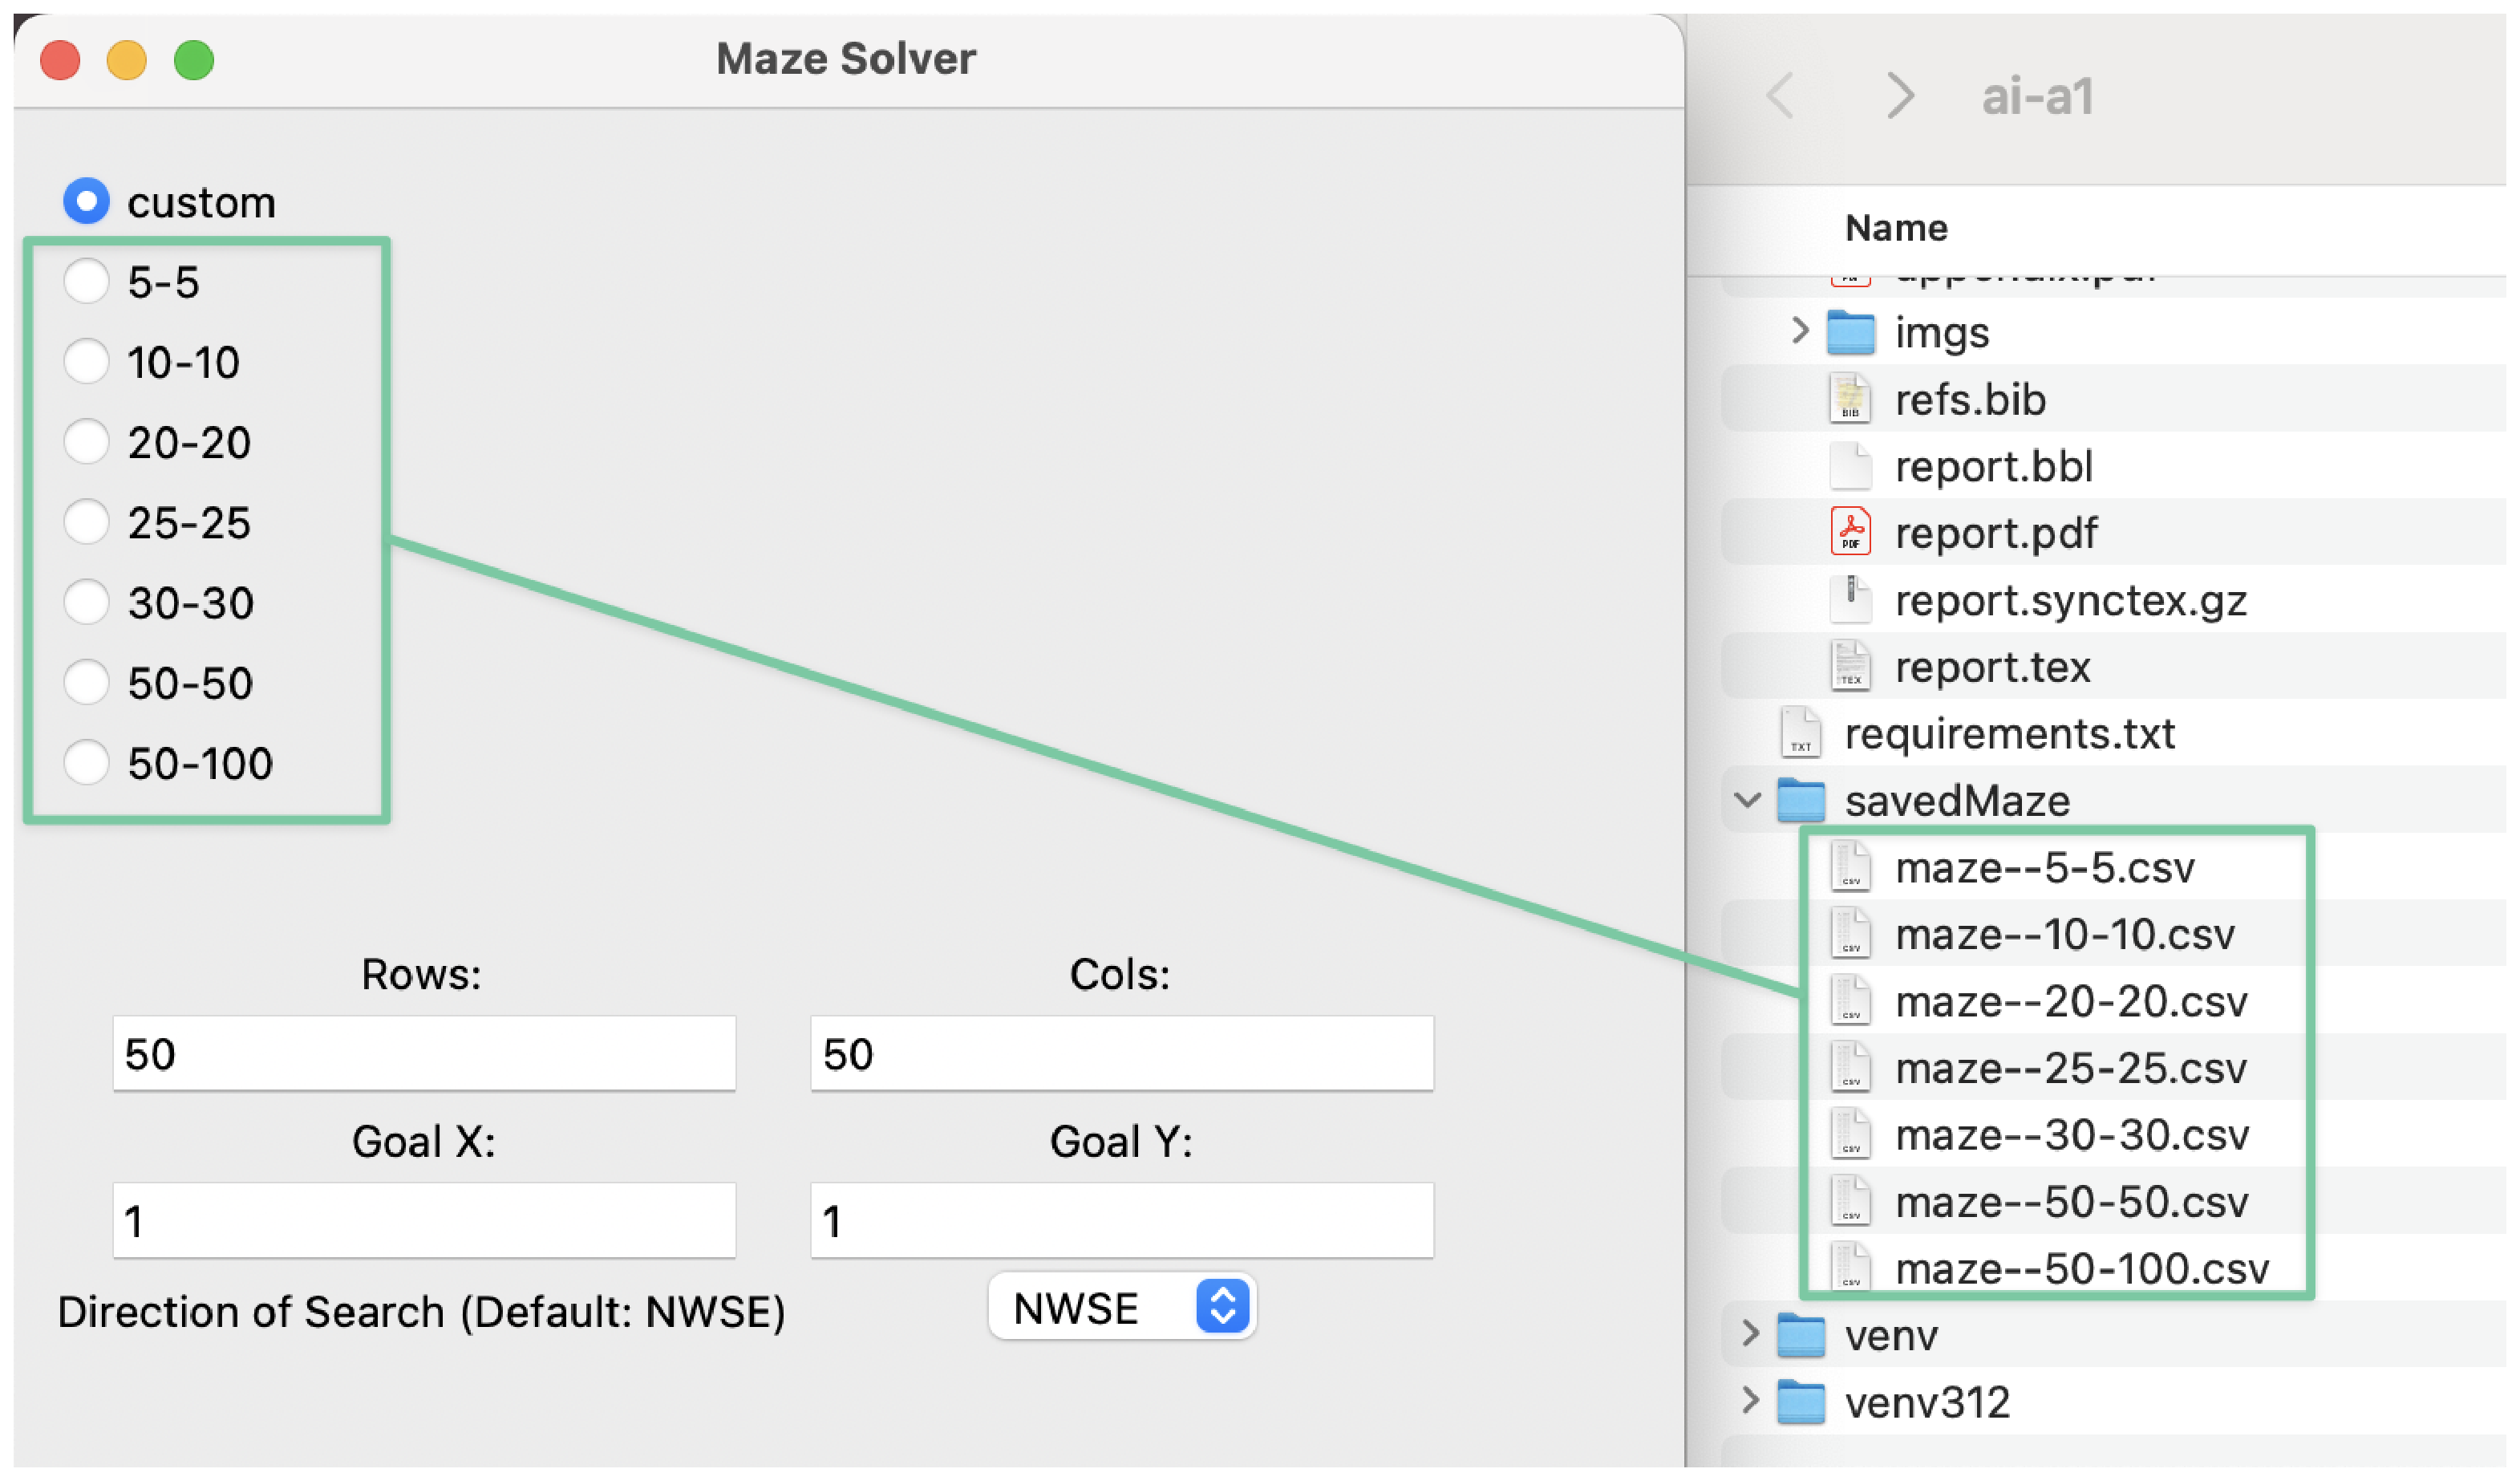
\includegraphics[scale=0.148]{imgs/auto_load.eps}
    \caption{Auto Load Saved Maze From \texttt{savedMaze}}
    \label{figure}
\end{figure}

I have tried with different sizes of mazes, including: \texttt{5x5}, \texttt{10x10}, \texttt{20x20}, \texttt{25x25} \texttt{30x30}, \texttt{40x40}, \texttt{50x50}, \texttt{75x75}, \texttt{50x100}.
For some mazes that size over \texttt{75x75}, some algorithms failed to get the correct final path for the maze. 
Since the goal is to analyze the performance of different algorithms generally, the mazes with size \texttt{5x5}, \texttt{20x20}, \texttt{30x30}, \texttt{50x50}, \texttt{50x100} are used to evaluate the performance of the algorithms in this assignment.
Thus, those selected maze will be evaluated in the following sections, Figure 2 is the screenshot of those mazes.
\begin{figure}[h]
    \centering
    \begin{subfigure}[b]{0.3\textwidth}
        \centering
        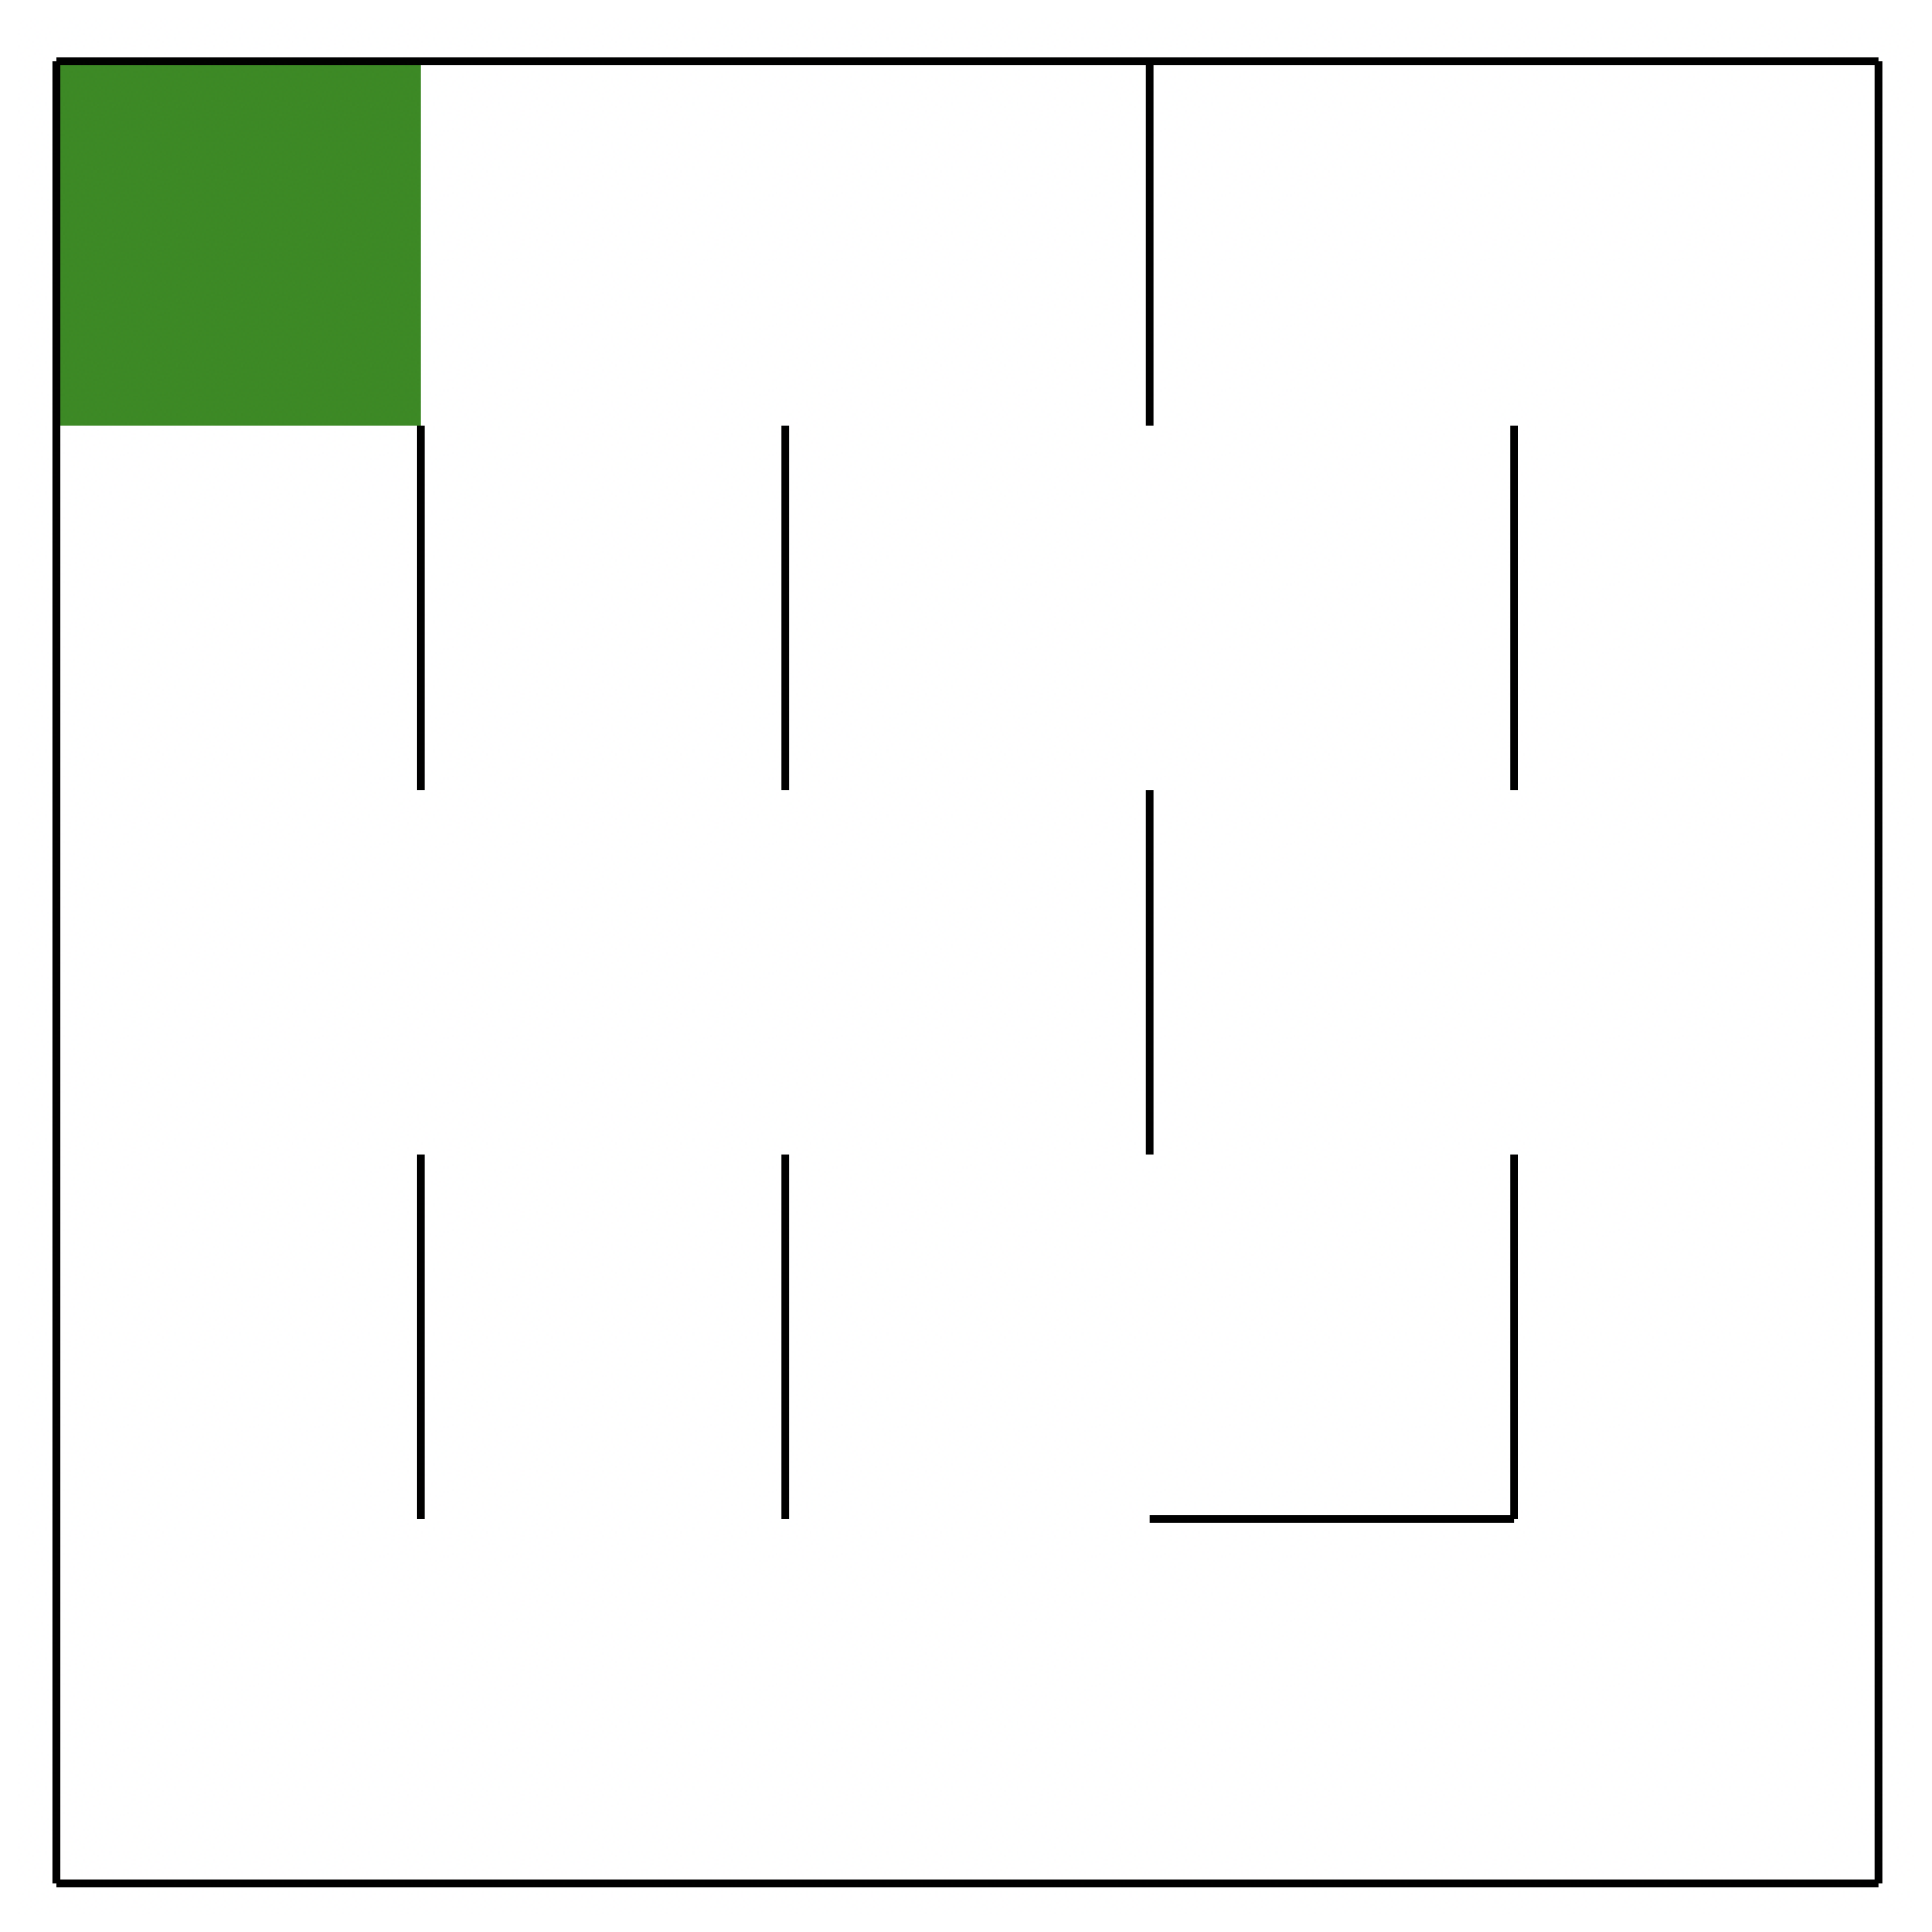
\includegraphics[width=\textwidth]{imgs/5x5.eps}
        \caption{5x5}
    \end{subfigure}
    \begin{subfigure}[b]{0.3\textwidth}
        \centering
        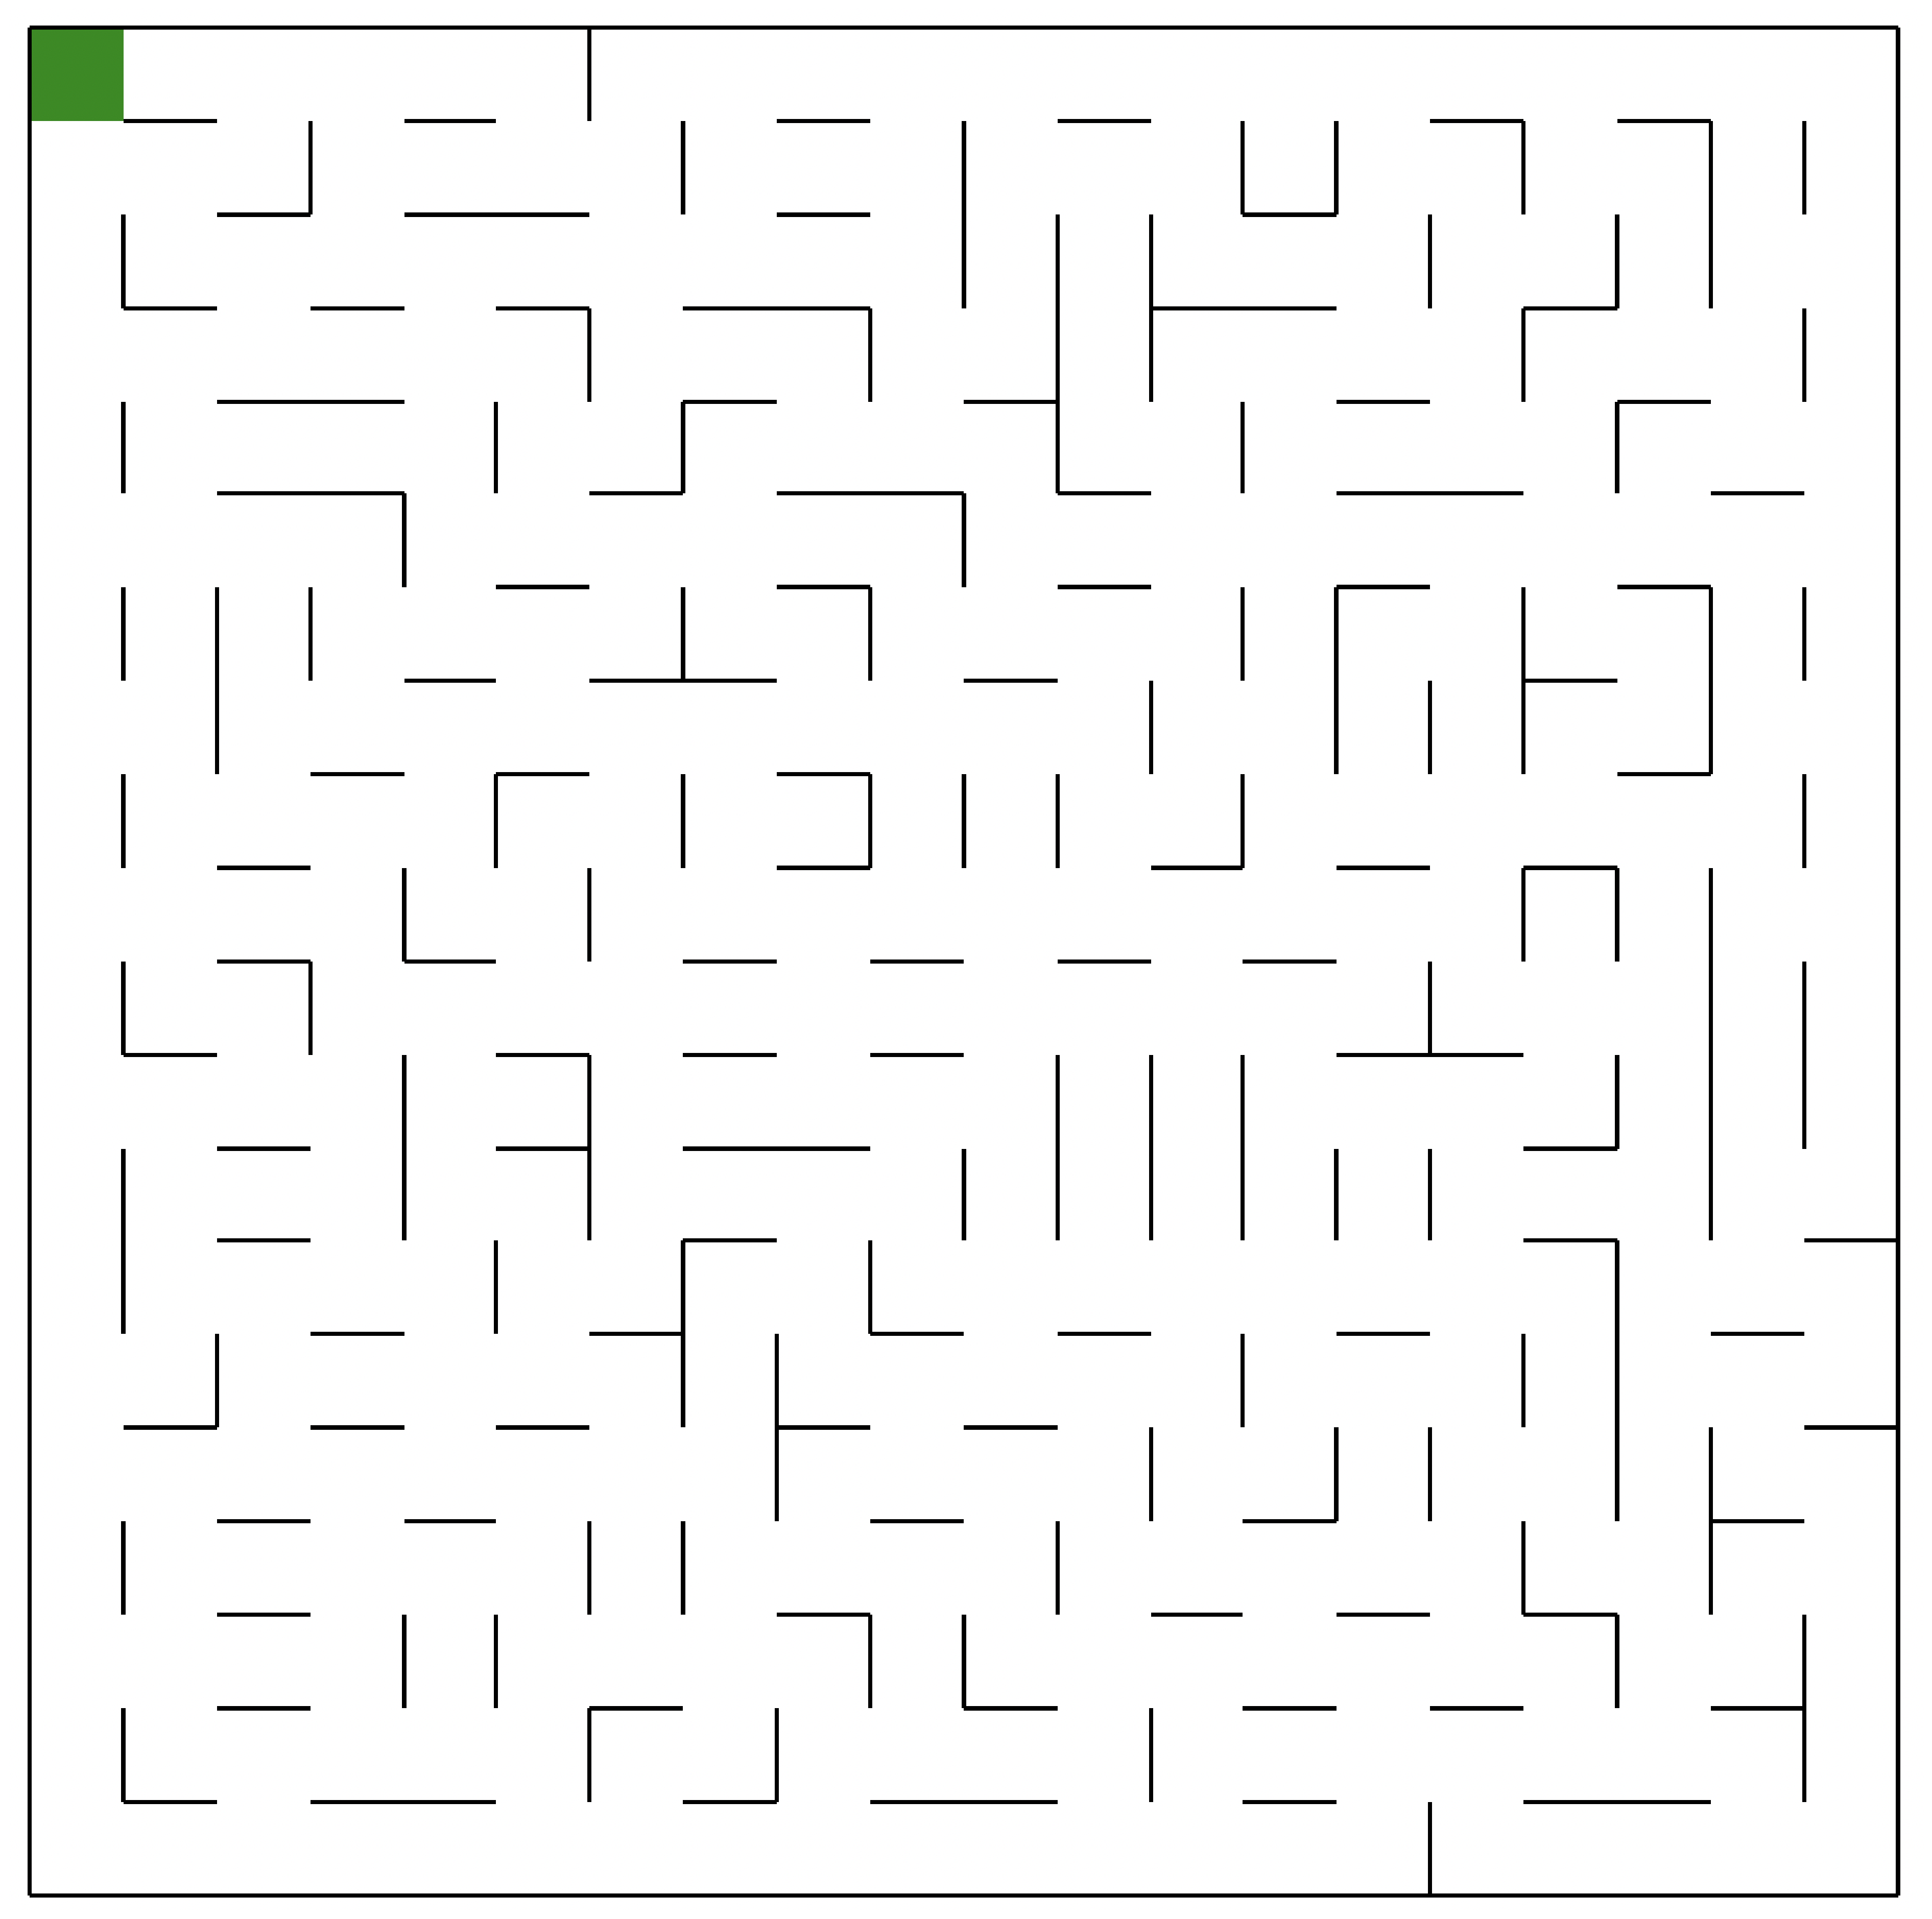
\includegraphics[width=\textwidth]{imgs/20x20.eps}
        \caption{20x20}
    \end{subfigure}
    \begin{subfigure}[b]{0.3\textwidth}
        \centering
        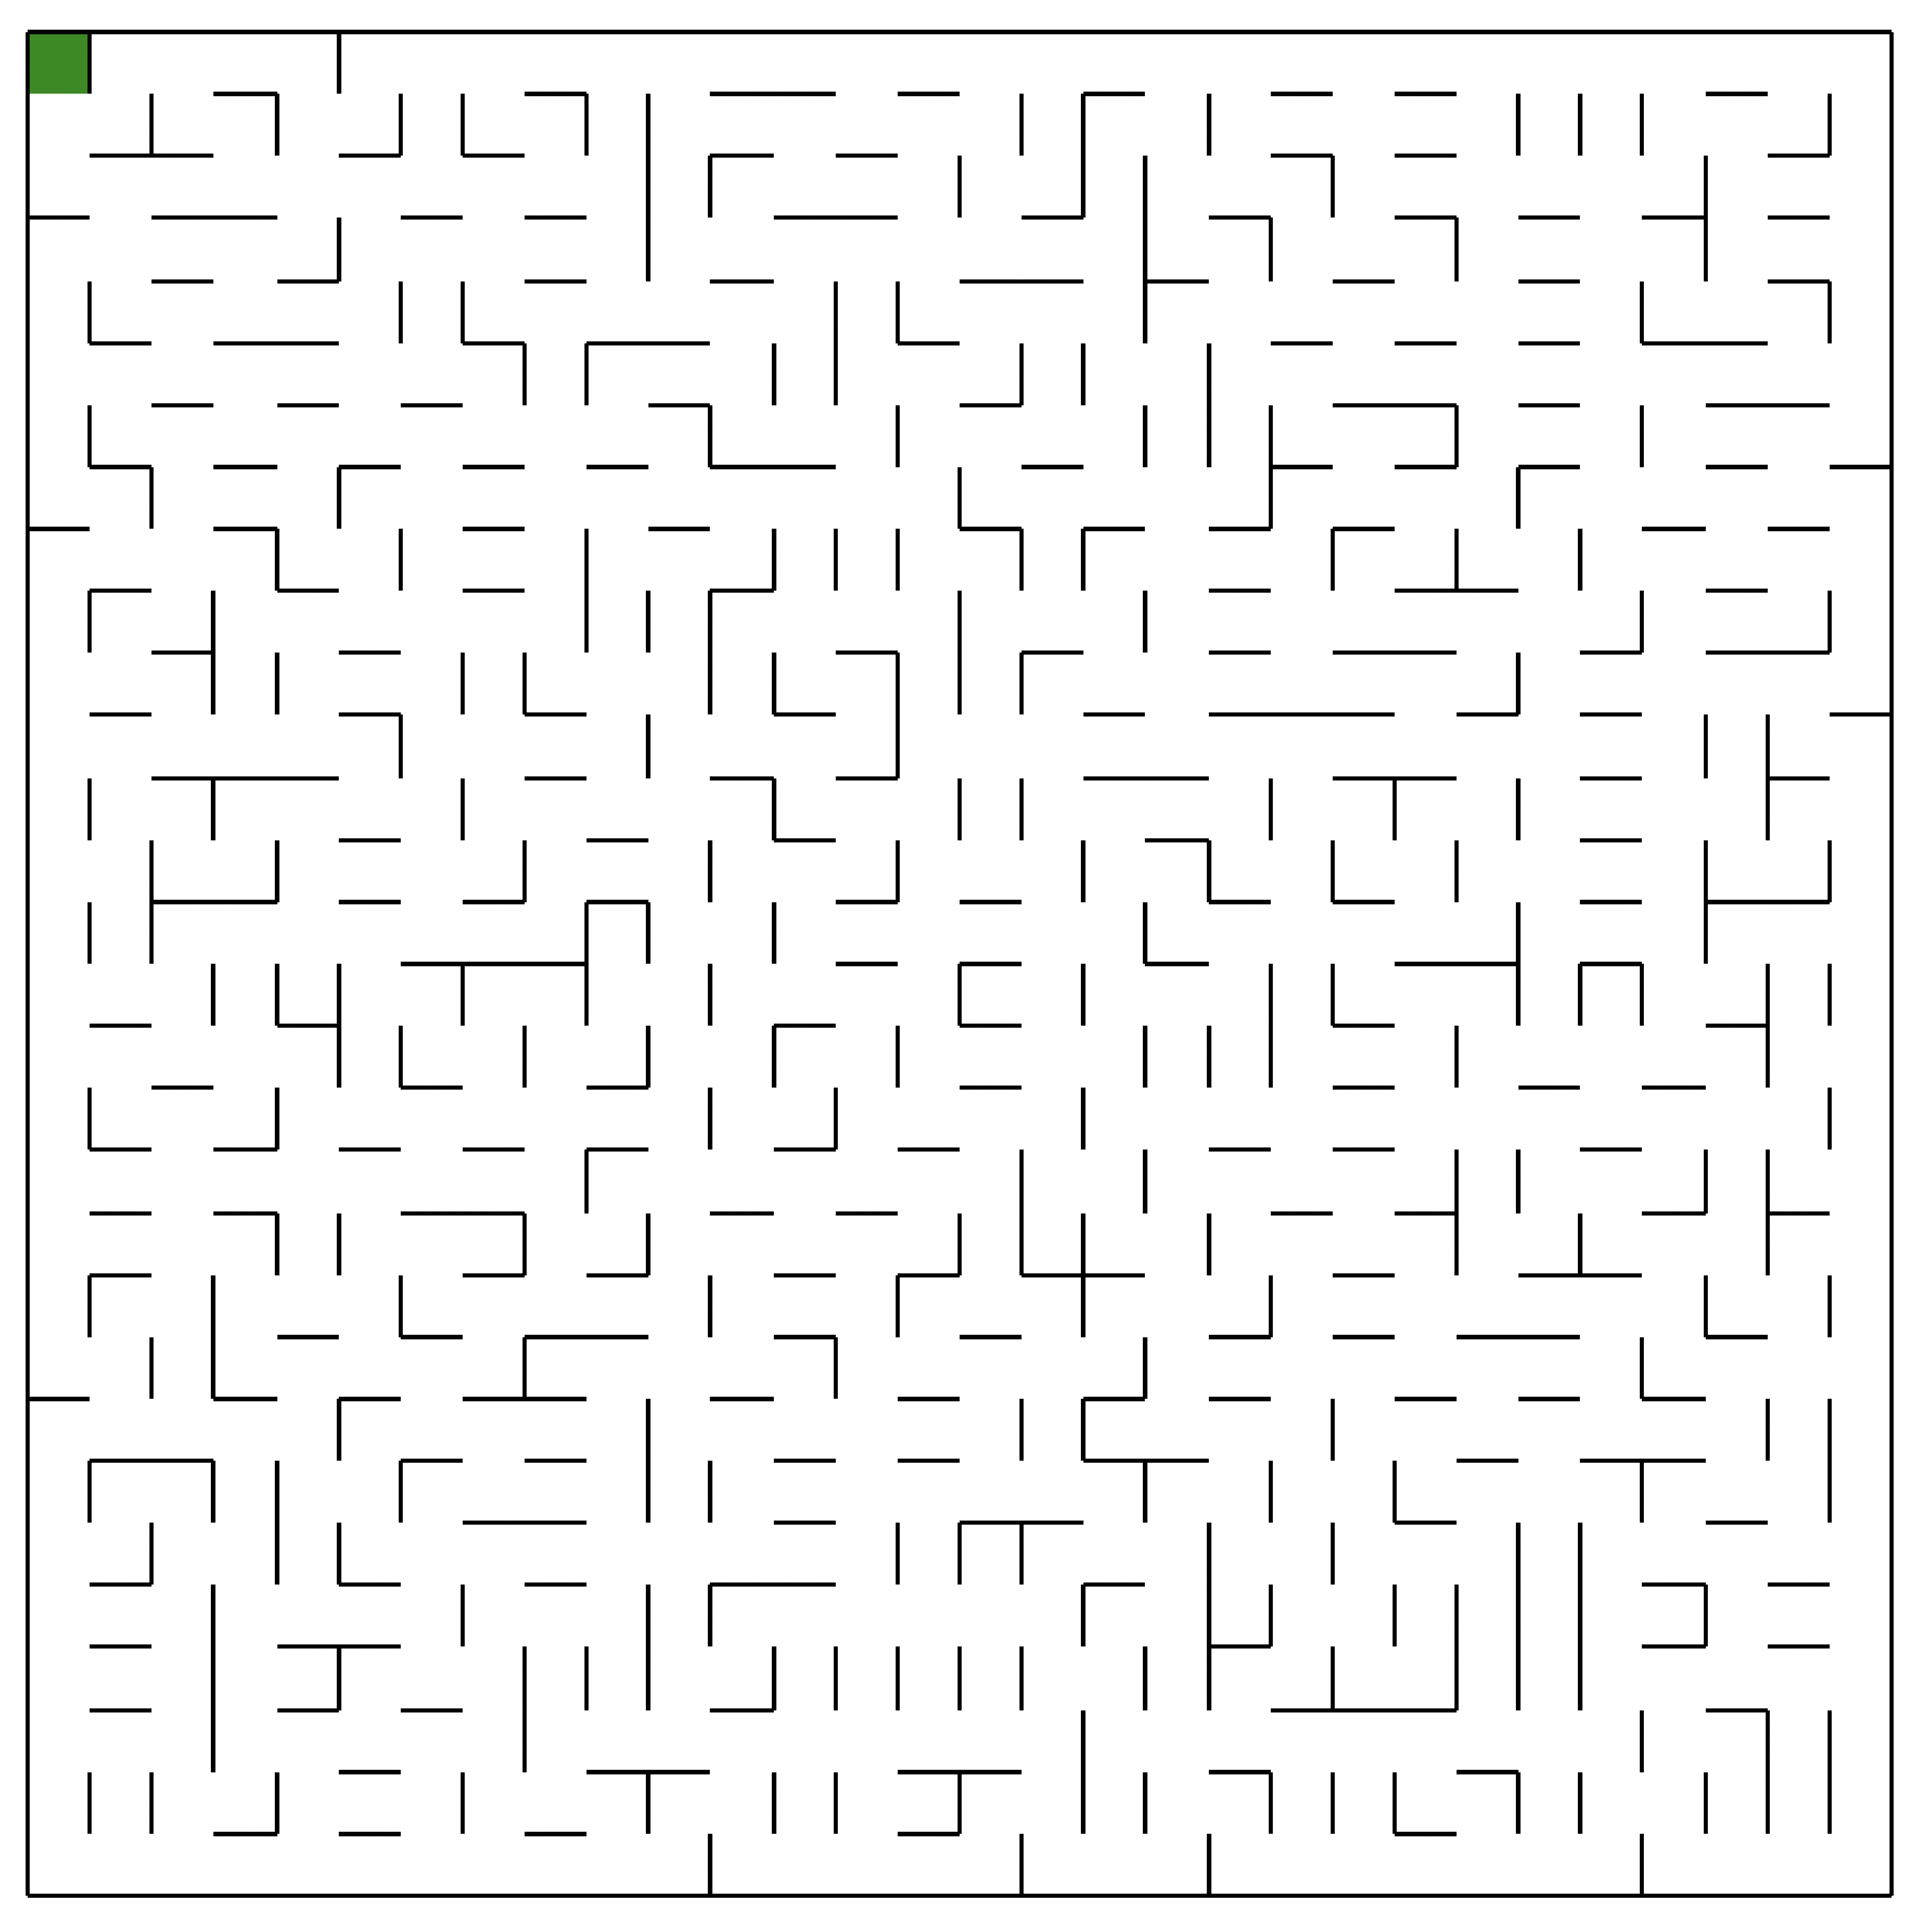
\includegraphics[width=\textwidth]{imgs/30x30.eps}
        \caption{30x30}
    \end{subfigure}
    \newline
    \begin{subfigure}[b]{0.3\textwidth}
        \centering
        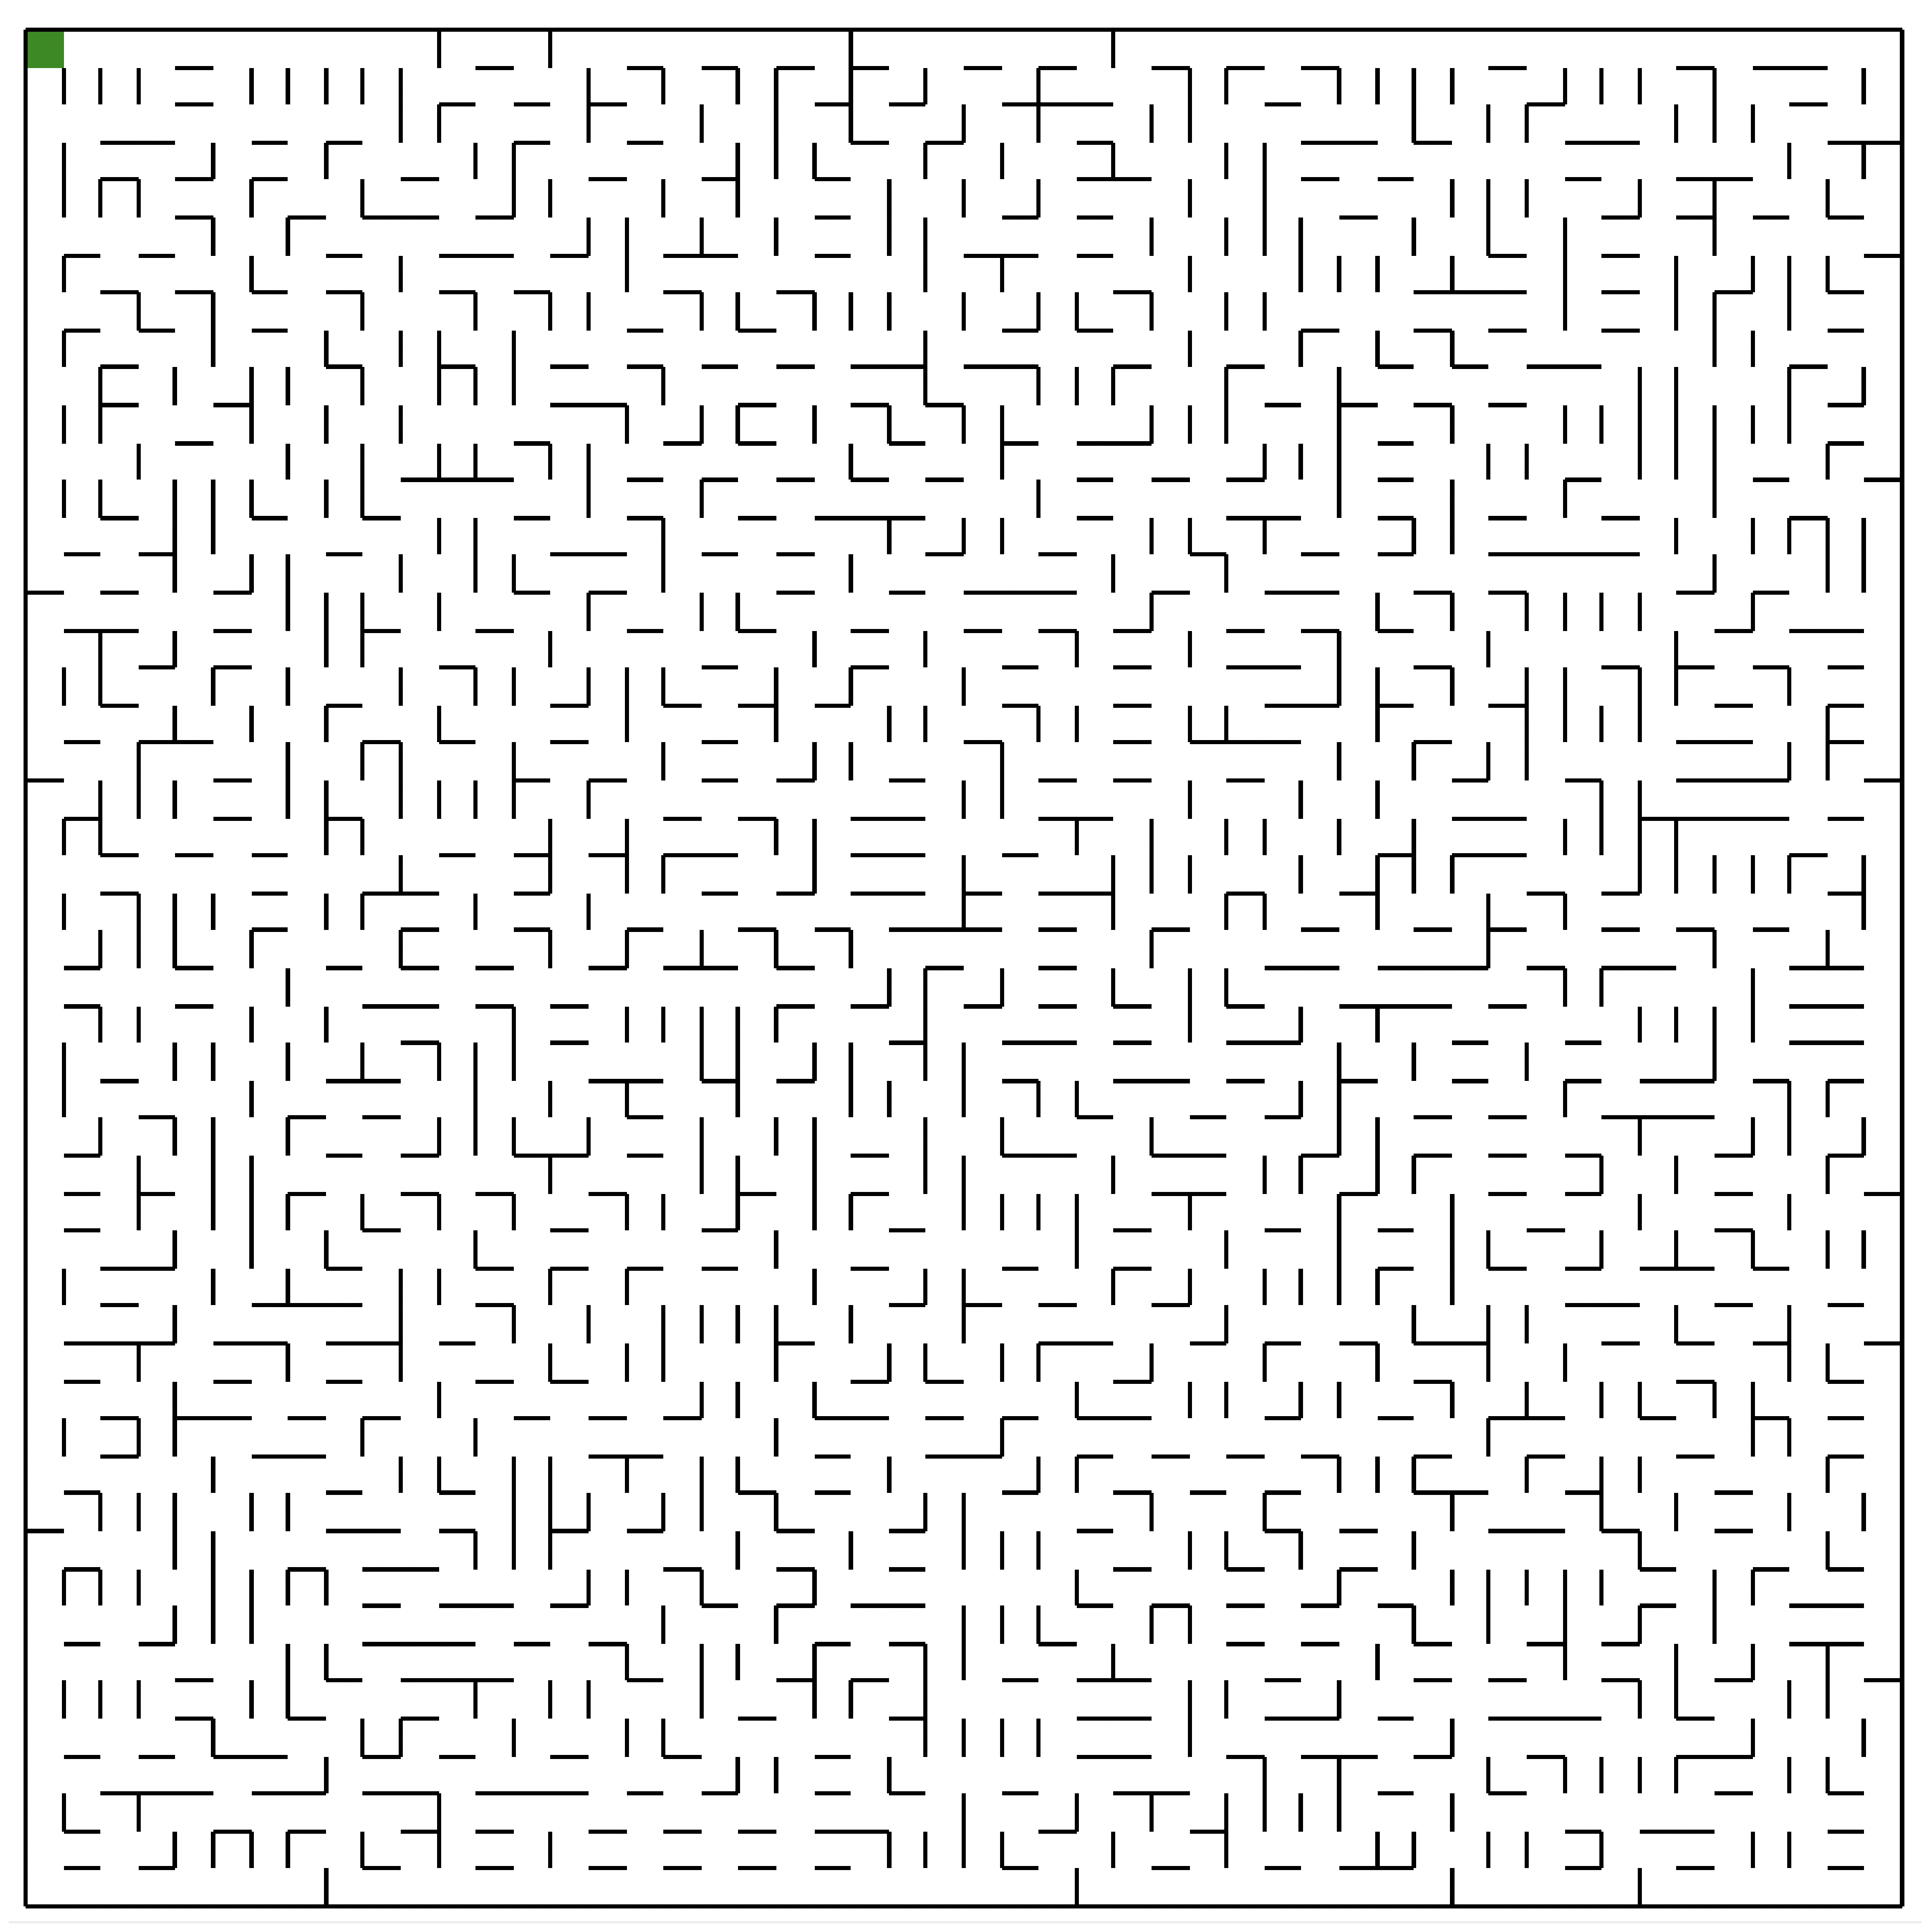
\includegraphics[width=\textwidth]{imgs/50x50.eps}
        \caption{50x50}
    \end{subfigure}
    \begin{subfigure}[b]{0.6\textwidth}
        \centering
        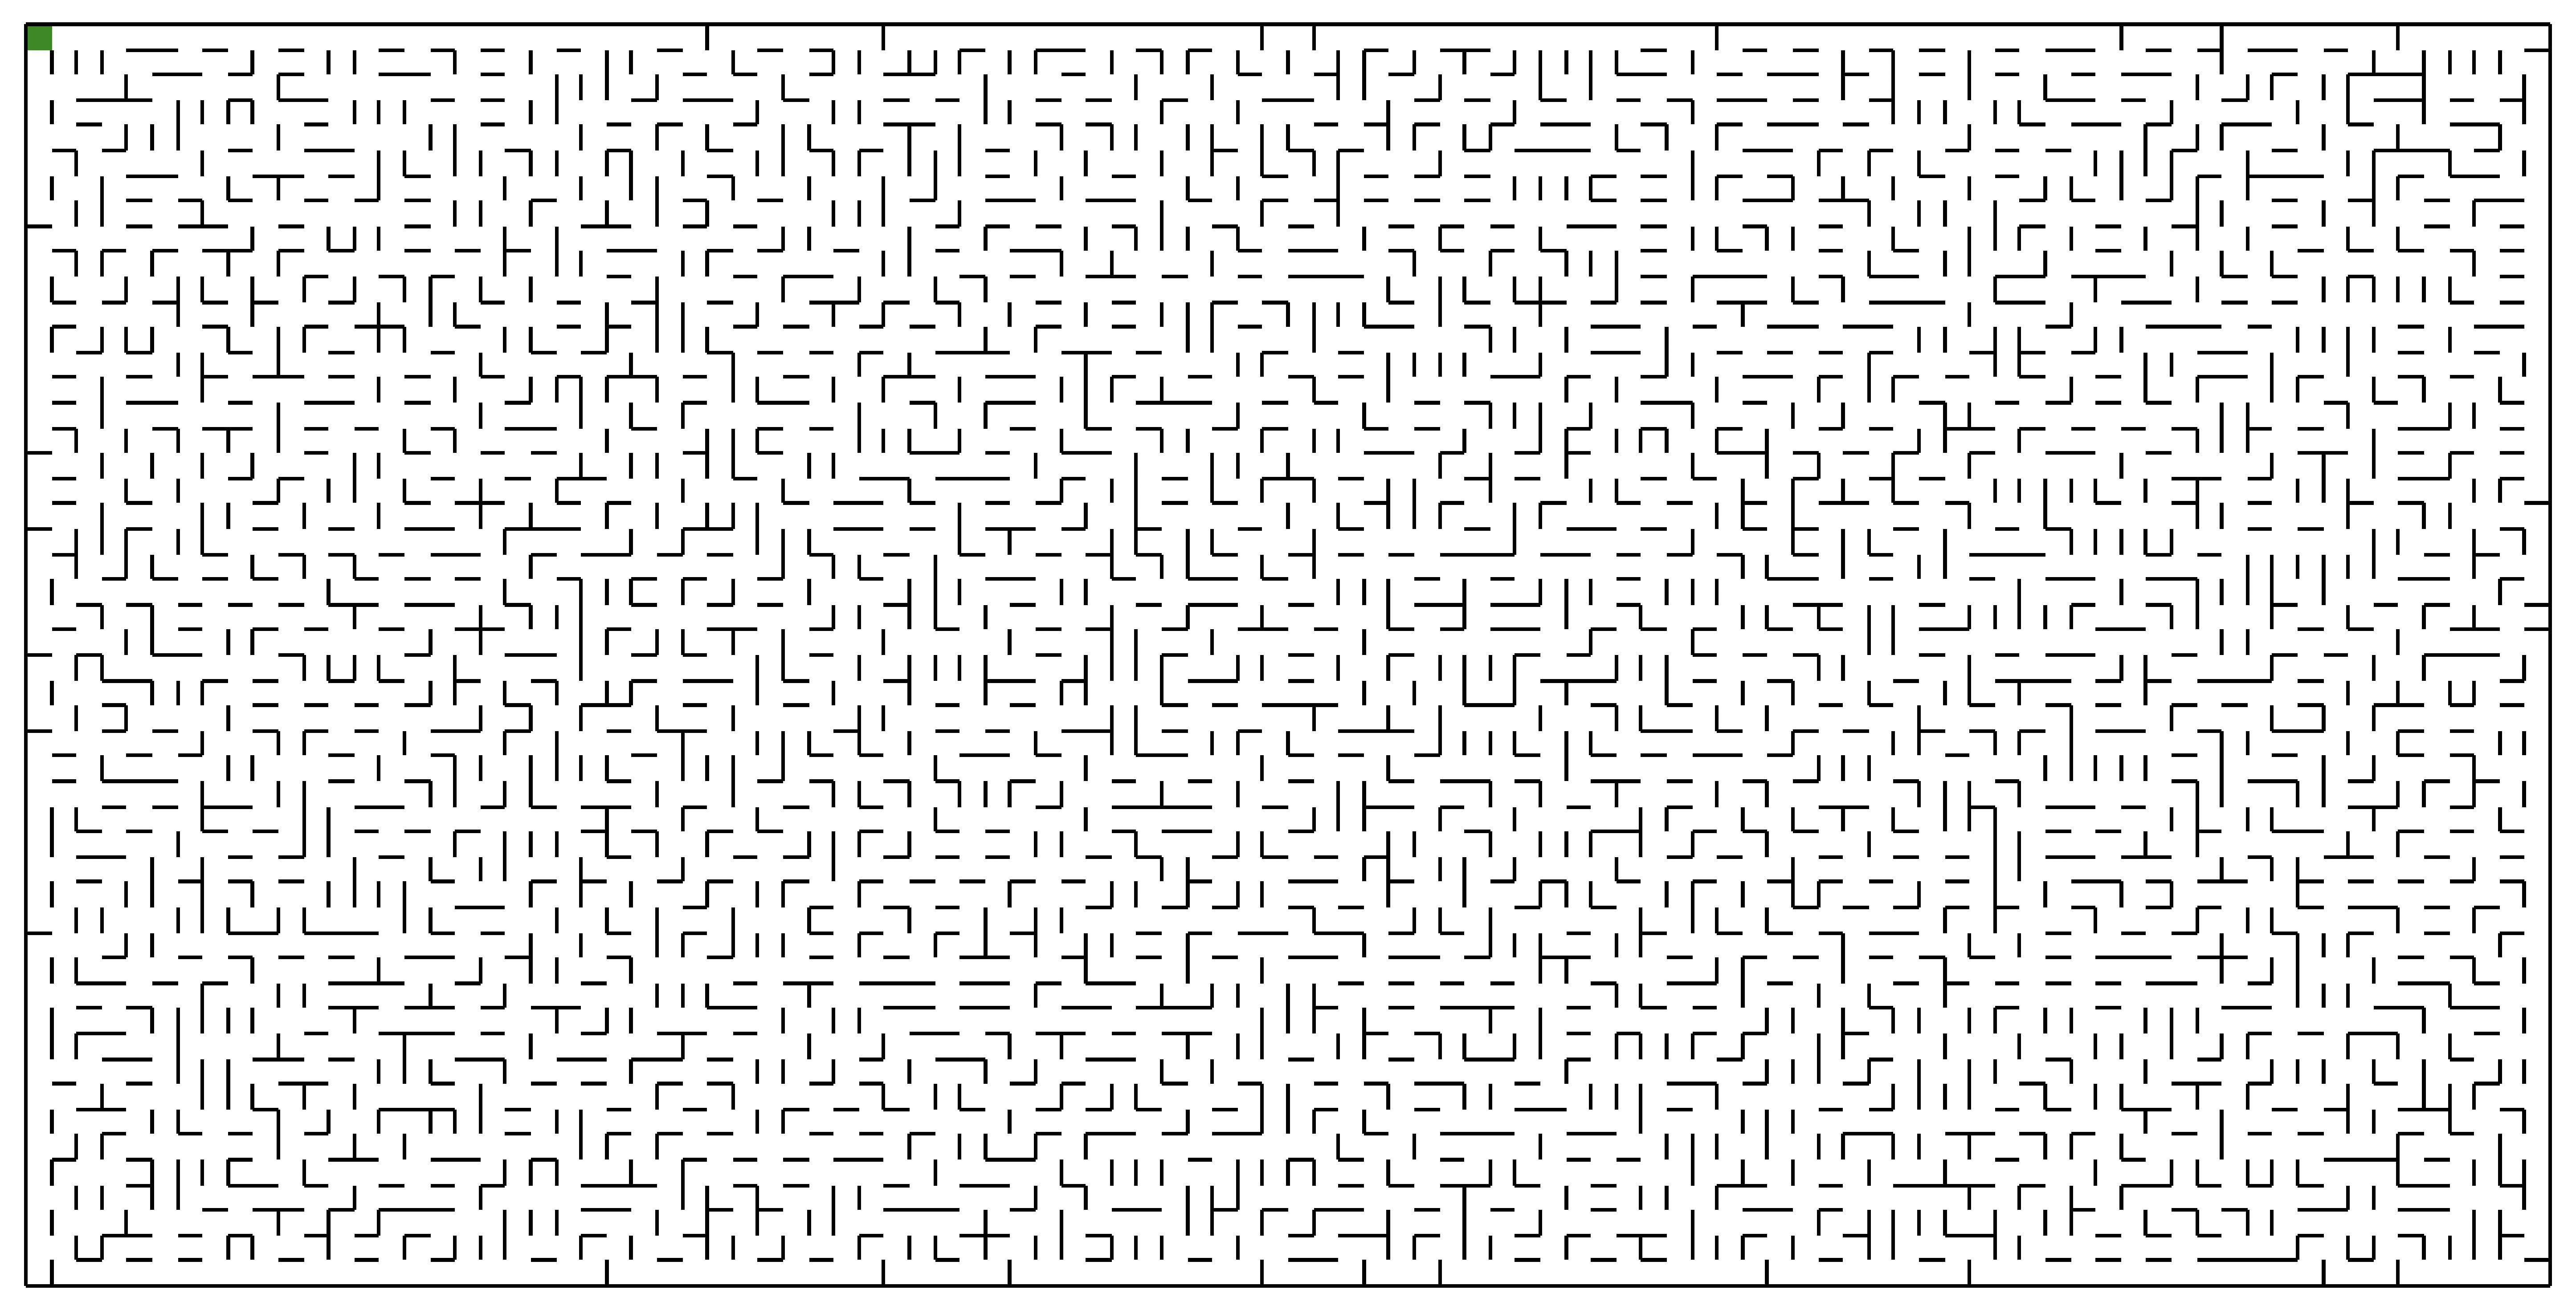
\includegraphics[width=\textwidth]{imgs/50x100.eps}
        \caption{50x100}
    \end{subfigure}
    \caption{Used Maze}
\end{figure}

\subsection{GUI}
I've programed a GUI for ease of use.
 The GUI has the capability to show the maze saved in \texttt{savedMaze} folder as some checkboxes. Instead of choosing the saved maze, the user can also generate a random maze by specifying the size of the maze.
 For any type of maze, the user can choose the goal of the maze, the search direction of search algorithms, and the algorithm to solve the maze. For the three search algorithms, the user can choose to show the search path of the algorithms or not. For this option, the solver will show the search path firstly(then will disappear), then show the final path.
 When click \texttt{run} button, the algorithms selected will be used to calculated the path and the pyamaze will show the final path, and the performance of the algorithms will be shown in the GUI as label. 

 Besides, when select the algorithms, there will also be some figures shown from the matplotlib library to visulize the performance of the algorithms. The figure will show the path steps (includ the start node and the goal node), time cost(in milliseconds), and the memory peak(in MB) for each selected algorithm. For graph search algorithms, there will also be a figure to show the search path steps of the maze. For the MDP algorithms, there will also be a figure to show the heat map of each node after the iteration.
 Those figure will be used for the evaluation later in this report. The figure will automatically saved to the \texttt{imgaes} folder as \texttt{.eps} file for the ease of use.
 \begin{figure}[htbp]
    \centering
    \begin{subfigure}{0.34\textwidth}

        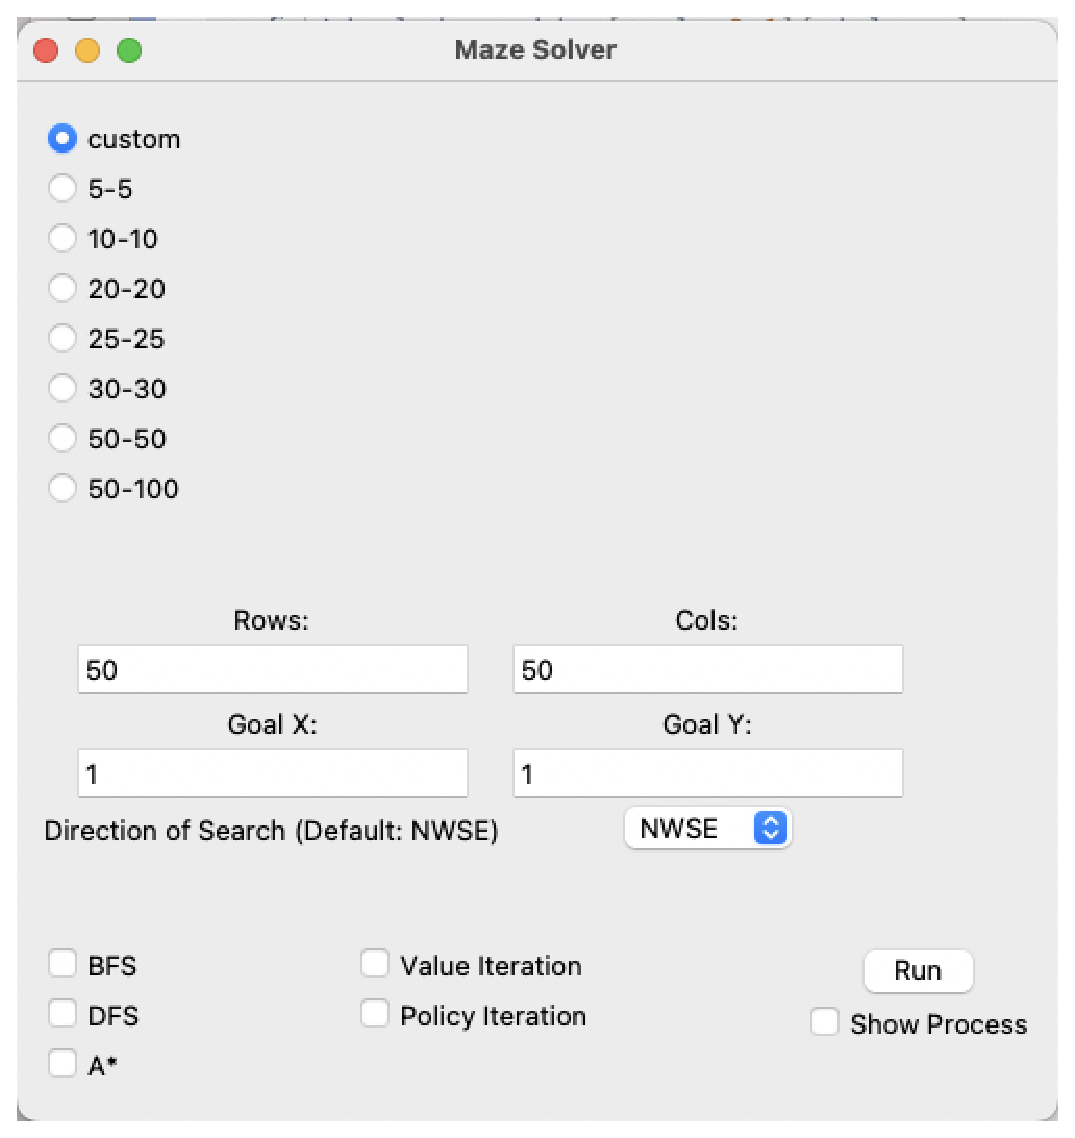
\includegraphics[width=\textwidth]{imgs/mainGUI.eps}
        \caption{main GUI}
    \end{subfigure}
    \\
    \begin{subfigure}{1.0\textwidth}
        \centering
        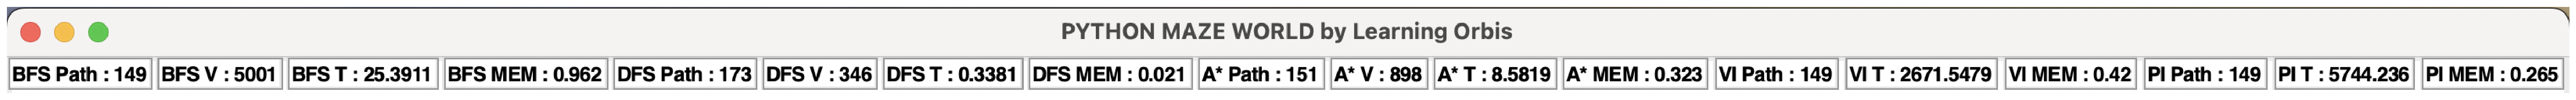
\includegraphics[width=\textwidth]{imgs/label.eps}
        \caption{labels in maze}
    \end{subfigure}
    \caption{GUI of the program}
\end{figure}

\section{Algorithms}
In this assignment, I've developed five different algorithms to solve the maze. 
For better reuse of the code, I've created classes for each algorithm.
The algorithms are: Breadth First Search(BFS), Depth First Search(DFS), A* Search, Value Iteration, and Policy Iteration.
The BFS, DFS and A* is based on the same parent class \texttt{GraphSearchAlgorithms} and the Value Iteration and Policy Iteration algorithms are based on the same parent class \texttt{MarkovDecisionProcess}.
To use each class of algorithms, it is required to create an instance of the class with maze parameter \texttt{m} (import from pyamaze) and goal parameter \texttt{goal} (tuple). 
\subsection{Graph Search Algorithms}

\texttt{GraphSearchAlgorithms} is the the base class for the BFS, DFS and A* algorithms. This class initializes some data structures and methods that are used by the three algorithms. 

In this class, \texttt{start\_memory\_tracing} and \texttt{stop\_memory\_tracing} are used to trace and return the memory peak of the algorithm to \texttt{self.memory\_peak}. \texttt{validate\_node} is used to validate if the specific node is inside the maze and if it is visited.
\texttt{compute\_next\_node} works with \texttt{validate\_node} to calculate the next node of current node. \texttt{traceback\_final\_path} is used to trace back the dictionary \texttt{self.origin\_dict} to get the final path of the maze. \texttt{execute\_algorithm} is defined as an abstract method to be implemented by the child class. 
\texttt{get\_final\_path} is defined to get the \texttt{final path}, \texttt{search path}, \texttt{cost time} and \texttt{memory peak} of the algorithms. 

\subsubsection{Breadth First Search}
\texttt{BFS} is the child class of \texttt{GraphSearchAlgorithms}. 
This class will be initialized with the variables and methods inherited from the parent class, and the start node will be put into \texttt{queue}.

\texttt{execute\_algorithm} is the main method of this class. 
It execute the BFS algorithm and trace the time and memory for evaluation.
This method uses \texttt{queue} to store all the pending nodes.
This method works with \texttt{compute\_next\_node} to iterate each neighbors of current node. 
The final path is gotten from \texttt{traceback\_final\_path}.
\subsubsection{Depth First Search}
\texttt{DFS} is the child class of \texttt{GraphSearchAlgorithms}. 
This class will be initialized with the variables and methods inherited from the parent class. 
When initializing, \texttt{start node} will be put into \texttt{final path} and \texttt{search path}.

\texttt{execute\_algorithm} is the main method of this class. 
It execute the DFS algorithm and trace the time and memory for evaluation.
Instead of using queue in BFS, this method uses \texttt{final path} as a stack to store all the pending nodes.
This method also works with \texttt{compute\_next\_node} to iterate each neighbors of current node.
Also, the final path is gotten from \texttt{traceback\_final\_path}.

\subsubsection{A* Search}
\texttt{AStar} is the child class of \texttt{GraphSearchAlgorithms}.
This class will be initialized with the variables and methods inherited from the parent class. 
The \texttt{g socre} is initialized with a 0 g score start node. The \texttt{priority queue} is also initialized to used to manage nodes during the search based on their total cost.

The \texttt{h\_score} method is used to calculate the heuristic cost of the node. It will check if the \texttt{manhattan\_flag} is True or False.
If it is True, the method will calculate the manhattan distance between the node and the goal node. If it is False, the method will calculate the euclidean distance between the node and the goal node. 
While Euclidean distance may overestimate and lead to A* algorithm choosing a suboptimal path, Manhattan distance does not overestimate the actual distance to the target in a maze that can only move up, down\cite{AStarSearch} \cite{m_and_e}. 
Thus, the manhattan distance is used in this assignment. 

\texttt{execute\_algorithm} is the main method of this class. 
It execute the A* algorithm and trace the time and memory for evaluation.
This algorithm is based on the \texttt{priority queue}. 
This algorithm calculates the cost of the next node and compares it within a while loop
Also, the final path is gotten from \texttt{traceback\_final\_path}.

\subsection{Markov Decision Process}
\texttt{MarkovDecisionProcess} is the the base class for the value iteration and policy iteration algorithms. 
This class initializes some data structures and methods that are used by the two algorithms. 
In this class, \texttt{start\_memory\_tracing} and \texttt{stop\_memory\_tracing} are used to trace and return the memory peak of the algorithm to \texttt{self.memory\_peak}. 
\texttt{get\_final\_path} is defined to get the \texttt{final path}, \texttt{cost time} and \texttt{memory peak} of the algorithms. 

\texttt{discount factor} and \texttt{convergence threshold} are set to \texttt{0.9} and \texttt{0.000001} respectively in this assignment.
Those two are important parameters for the MDP algorithms. I've tried with different values such as 0.1, 0.3, 0.5, 0.9 for discount factor, and found that \texttt{0.9} and \texttt{0.000001} are the best values for the performance of my MDP algorithms.

\texttt{get\_direction\_for\_current\_node} is used to get the direction of the current node when get the \texttt{final path}. This method is passed to the child class for implementation since that two iteration are not same.
\texttt{execute\_algorithm} is defined as an abstract method to be implemented by the child class either. 
\texttt{plot\_maze\_weights} is used to draw the heat map of the maze after the iteration.

\subsubsection{Value Iteration}
\texttt{ValueIteration} is the child class of \texttt{MarkovDecisionProcess}.
This class will be initialized with the variables and methods inherited from the parent class.
Value iteration is initialized by setting the transition value to \texttt{10} for the goal node and \texttt{0} for all other nodes.
Also, the transition reward is initialized to \texttt{100} for the goal node and 0 for all other nodes.

\texttt{get\_direction\_for\_current\_node} return data based on \texttt{max(current\_node, key=current\_node.get)} and \texttt{transition\_dictionary}.
\texttt{execute\_iteration} is the main method of this class. 
This method updates the value of each node with constant iterations until the convergence condition is reached. 
The mathematical formulas that can be referred to are:
\[ V(s) = \max_{a \in A} \left\{ R(s, a) + \gamma \sum_{s' \in S} P(s'|s, a) V(s') \right\} \]
Which is calculated by using code:

\begin{lstlisting}
    next_transition_value = self.transition_probability[direction] * (self.transition_reward[current_node] + self.discount_factor * self.transition_value[next_node])
    temp_transition_value.append(next_transition_value)
    self.transition_dictionary[current_node][direction] = next_transition_value
    best_transition_value = max(temp_transition_value)
\end{lstlisting}

\subsubsection{Policy Iteration}
\texttt{PolicyIteration} is the child class of \texttt{MarkovDecisionProcess}.
This class will be initialized with the variables and methods inherited from the parent class.
Policy Iteration algorithm is initialized by setting the transition value and reward to \texttt{1} for the goal node and \texttt{0} for all other nodes.
The default \texttt{policy} is set to \texttt{N} (North/Up).

\texttt{get\_direction\_for\_current\_node} return data based on \texttt{policy} direction.
     is defined to conduct the policy evaluation based on the mathematical formula:
\[ V^{\pi}(s) = R(s, \pi(s)) + \gamma \sum_{s' \in S} P(s'|s, \pi(s)) V^{\pi}(s') \]
Which is calculated by using code:
\begin{lstlisting}
    temp_node_transition_value[current_node][direction] = self.transition_probability[direction] * (self.transition_reward[current_node] + self.discount_factor * next_transition_value)
    self.transition_dictionary[current_node][current_policy] = (self.transition_probability[current_policy] * (self.transition_reward[current_node] + next_transition_value * self.discount_factor))
    if abs(self.transition_value[current_node] - (self.transition_probability[current_policy] * (self.transition_reward[current_node] + next_transition_value * self.discount_factor))) > self.convergence_threshold:
        self.transition_value[current_node] = self.transition_probability[current_policy] * (self.transition_reward[current_node] + next_transition_value * self.discount_factor)
        value_converged_flag = False
\end{lstlisting}

\texttt{execute\_iteration} is the main method of this class. It updates the value of each node by doing policy evaluation with \texttt{calculate\_transition\_value} and then performs the policy improvement.
The policy improvement is based on the mathematical formula:
\[ \pi'(s) = \arg \max_{a \in A} \left\{ R(s, a) + \gamma \sum_{s' \in S} P(s'|s, a) V^{\pi}(s') \right\} \]
Which is calculated by using code:
\begin{lstlisting}
    for current_node in self.m.grid:
    if current_node == self.goal:
        continue
    current_node_transition_value = self.calculate_transition_value(current_node)
    current_node_transition_policy = get_direction(current_node_transition_value[current_node])
    if current_node_transition_policy != self.policy[current_node]:
        self.policy[current_node] = current_node_transition_policy
        policy_converged_flag = False
\end{lstlisting}
Policy evaluation and policy improvement are alternated until the policy converges.

\section{Evaluation}
Table 1 summarizes the performance of the algorithms on the selected mazes. 
It can be discovered that the DFS algorithm has the best performance in terms of time and memory, however, the path length is the longest. 
This is because the DFS algorithm tends to explore a branch of the maze in depth until a dead end is reached or a goal is found, a strategy that is not always effective in finding the shortest path, but accomplishes the search task with low computational time and memory consumption.
Also, somtimes the A* algorithm has the best performance in terms of visited nodes. To have a better understanding of the performance, the following sections will use figure to analyze.
\begin{table}[H]
    \centering
    \label{tab:performance}
    \begin{tabular}{cccccc}
    \toprule
    \textbf{Maze Size} & \textbf{Algorithm} & \textbf{Path Length} & \textbf{Calculated Time (ms)} & \textbf{Memory Peak (MB)} & \textbf{Visited Nodes} \\
    \midrule
    \multirow{5}{*}{5x5} & BFS & 9 & 0.2191 & 0.004 & 26 \\
                         & DFS & \textbf{11} & \textbf{0.0348} & \textbf{0.001} & 22 \\
                         & A* & 9 & 0.1507 & 0.005 & \textbf{15} \\
                         & VAL & 9 & 12.697 & 0.002 & - \\
                         & POL & 9 & 3.583 & 0.002 & - \\
    \midrule
    \multirow{5}{*}{20x20} & BFS & 39 & 2.3408 & 0.061 & 401 \\
                           & DFS & \textbf{45} & \textbf{0.1132} & \textbf{0.005} & 90 \\
                           & A* & 39 & 0.4311 & 0.02 & \textbf{49} \\
                           & VAL & 39 & 214.5798 & 0.034 & - \\
                           & POL & 39 & 102.3591 & 0.022 & - \\
    \midrule
    \multirow{5}{*}{30x30} & BFS & 59 & 5.2621 & 0.09 & 901 \\
                           & DFS & \textbf{63} & \textbf{0.1237} & \textbf{0.007} & \textbf{126} \\
                           & A* & 61 & 3.4239 & 0.101 & 326 \\
                           & VAL & 59 & 487.3381 & 0.076 & - \\
                           & POL & 59 & 334.6488 & 0.049 & - \\
    \midrule
    \multirow{5}{*}{50x50} & BFS & 99 & 13.545 & 0.244 & 2501 \\
                           & DFS & \textbf{123} & \textbf{0.2058} & \textbf{0.017} & 255 \\
                           & A* & 99 & 2.1842 & 0.104 & \textbf{243} \\
                           & VAL & 99 & 1335.9559 & 0.21 & - \\
                           & POL & 99 & 1554.523 & 0.136 & - \\
    \midrule
    \multirow{5}{*}{50x100} & BFS & 149 & 24.23 & 0.962 & 5001 \\
                            & DFS & \textbf{173} & \textbf{0.3977} & \textbf{0.021} & \textbf{346} \\
                            & A* & 151 & 7.443 & 0.323 & 898 \\
                            & VAL & 149 & 2660.815 & 0.42 & - \\
                            & POL & 149 & 6087.6012 & 0.265 & - \\
    \bottomrule
    \end{tabular}
    \caption{Maze Solving Algorithms Performance}
\end{table}
\subsection{Path Steps, Time, and Memory Comparsion}
Figure 4 shows the path steps, time, and memory comparsion of the algorithms on the selected mazes.
It can be found that A* algorithm is also efficient comparing to the other algorithms, especially when the size of maze is getting bigger and bigger in terms of time.
Overall, the efficiency of the graph search algorithms is better than the MDP algorithms.
It is because that the MDP is based on the iteration, and the iteration is time-consuming.

Comparing in MDP, the Policy Iteration is more efficient than the Value Iteration in terms of memory.
When considering the time, the Value Iteration is more efficient than the Policy Iteration when the maze is smaller than 50x50.
When the maze is bigger than 50x50, the Value Iteration is more efficient than the Policy Iteration in terms of time.

BFS is even less efficient than MDP mostly in terms of memory. This is probably because it iterates over all the nodes and the maze is not weighted.

For mazes with multiple solutions, BFS, A*, Value Iteration and Policy Iteration have the shortest paths. DFS has the longest path. This is the expected result.
\newpage
\begin{figure}[H]
    \centering
    \begin{subfigure}[b]{1\textwidth}
        \centering
        \includegraphics[width=0.75\textwidth]{imgs/Path-Time-Memory-5-5.eps}
        \caption{5x5}
    \end{subfigure}
    \newline
    \begin{subfigure}[b]{1\textwidth}
        \centering
        \includegraphics[width=0.75\textwidth]{imgs/Path-Time-Memory-20-20.eps}
        \caption{20x20}
    \end{subfigure}
    \newline
    \begin{subfigure}[b]{1\textwidth}
        \centering
        \includegraphics[width=0.75\textwidth]{imgs/Path-Time-Memory-30-30.eps}
        \caption{30x30}
    \end{subfigure}
    \newline
    \begin{subfigure}[b]{1\textwidth}
        \centering
        \includegraphics[width=0.75\textwidth]{imgs/Path-Time-Memory-50-50.eps}
        \caption{50x50}
    \end{subfigure}
    \newline
    \begin{subfigure}[b]{1\textwidth}
        \centering
        \includegraphics[width=0.75\textwidth]{imgs/Path-Time-Memory-50-100.eps}
        \caption{50x100}
    \end{subfigure}
    \caption{Path Steps, Time, and Memory Comparsion}
\end{figure}
\newpage

\subsection{Search Path Steps Comparsion for Graph Search Algorithms}
Figure 5 shows the search path steps comparsion of the graph search algorithms on the selected mazes. 

\begin{figure}[htbp]
    \centering
    \begin{subfigure}[b]{0.45\textwidth}
        \centering
        \includegraphics[width=\textwidth]{imgs/Visited-5-5.eps}
        \caption{5x5}
    \end{subfigure}
    \begin{subfigure}[b]{0.45\textwidth}
        \centering
        \includegraphics[width=\textwidth]{imgs/Visited-20-20.eps}
        \caption{20x20}
    \end{subfigure}
    \newline
    \begin{subfigure}[b]{0.45\textwidth}
        \centering
        \includegraphics[width=\textwidth]{imgs/Visited-30-30.eps}
        \caption{30x30}
    \end{subfigure}
    \begin{subfigure}[b]{0.45\textwidth}
        \centering
        \includegraphics[width=\textwidth]{imgs/Visited-50-50.eps}
        \caption{50x50}
    \end{subfigure}
    \newline
    \begin{subfigure}[b]{0.45\textwidth}
        \centering
        \includegraphics[width=\textwidth]{imgs/Visited-50-100.eps}
        \caption{50x100}
    \end{subfigure}
    \caption{Search Steps Comparsion}
\end{figure}
In most cases, A* and DFS explore the fewest nodes, BFS explores the most nodes.
\subsection{Heat Map for MDP Algorithms}
Figure 6 shows the heat map of the maze from MDP algorithms. This section is for visualizations.
\begin{figure}[hp]
    \centering
    \begin{subfigure}[b]{0.48\textwidth}
        \centering
        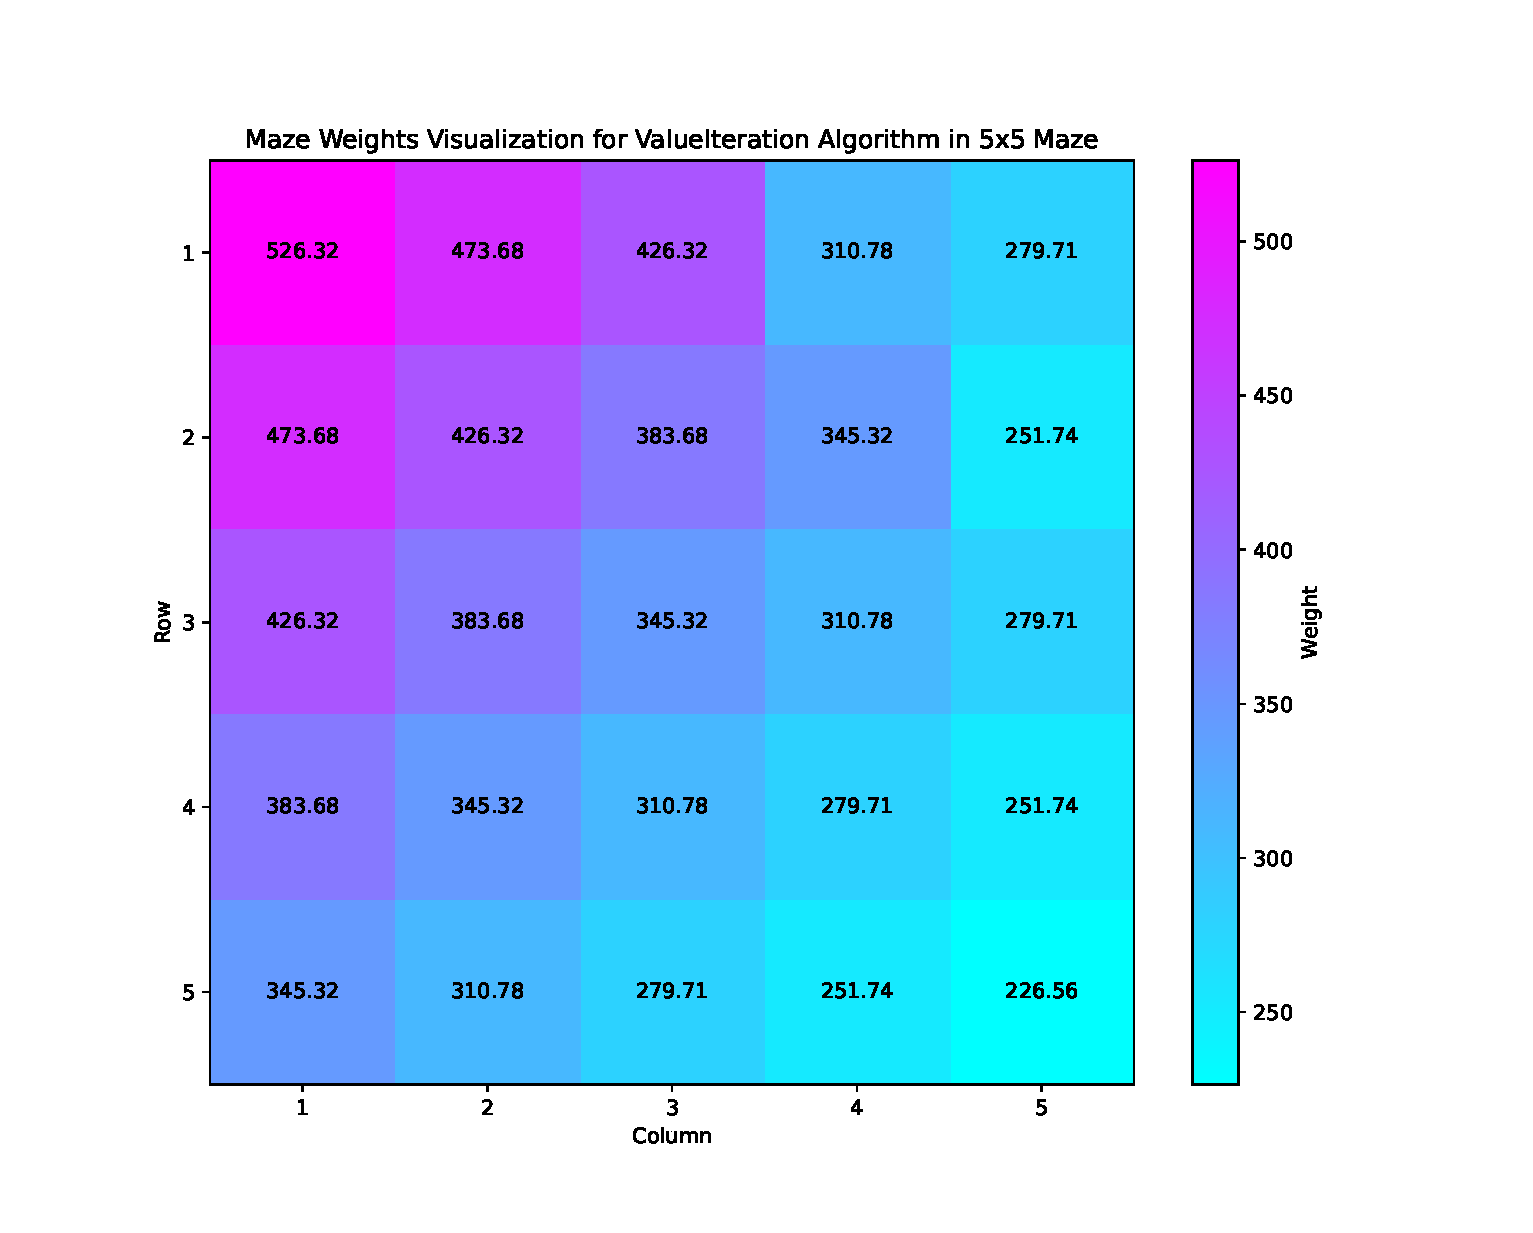
\includegraphics[width=\textwidth]{imgs/ValueIteration-5-5.eps}
        \caption{5x5 Value Iteration}
    \end{subfigure}
    \begin{subfigure}[b]{0.48\textwidth}
        \centering
        \includegraphics[width=\textwidth]{imgs/PolicyIteration-5-5.eps}
        \caption{5x5 Policy Iteration}
    \end{subfigure}
    \newline
    \begin{subfigure}[b]{0.48\textwidth}
        \centering
        \includegraphics[width=\textwidth]{imgs/ValueIteration-20-20.eps}
        \caption{20x20 Value Iteration}
    \end{subfigure}
    \begin{subfigure}[b]{0.48\textwidth}
        \centering
        \includegraphics[width=\textwidth]{imgs/PolicyIteration-20-20.eps}
        \caption{20x20 Policy Iteration}
    \end{subfigure}
    \newline
    \begin{subfigure}[b]{0.48\textwidth}
        \centering
        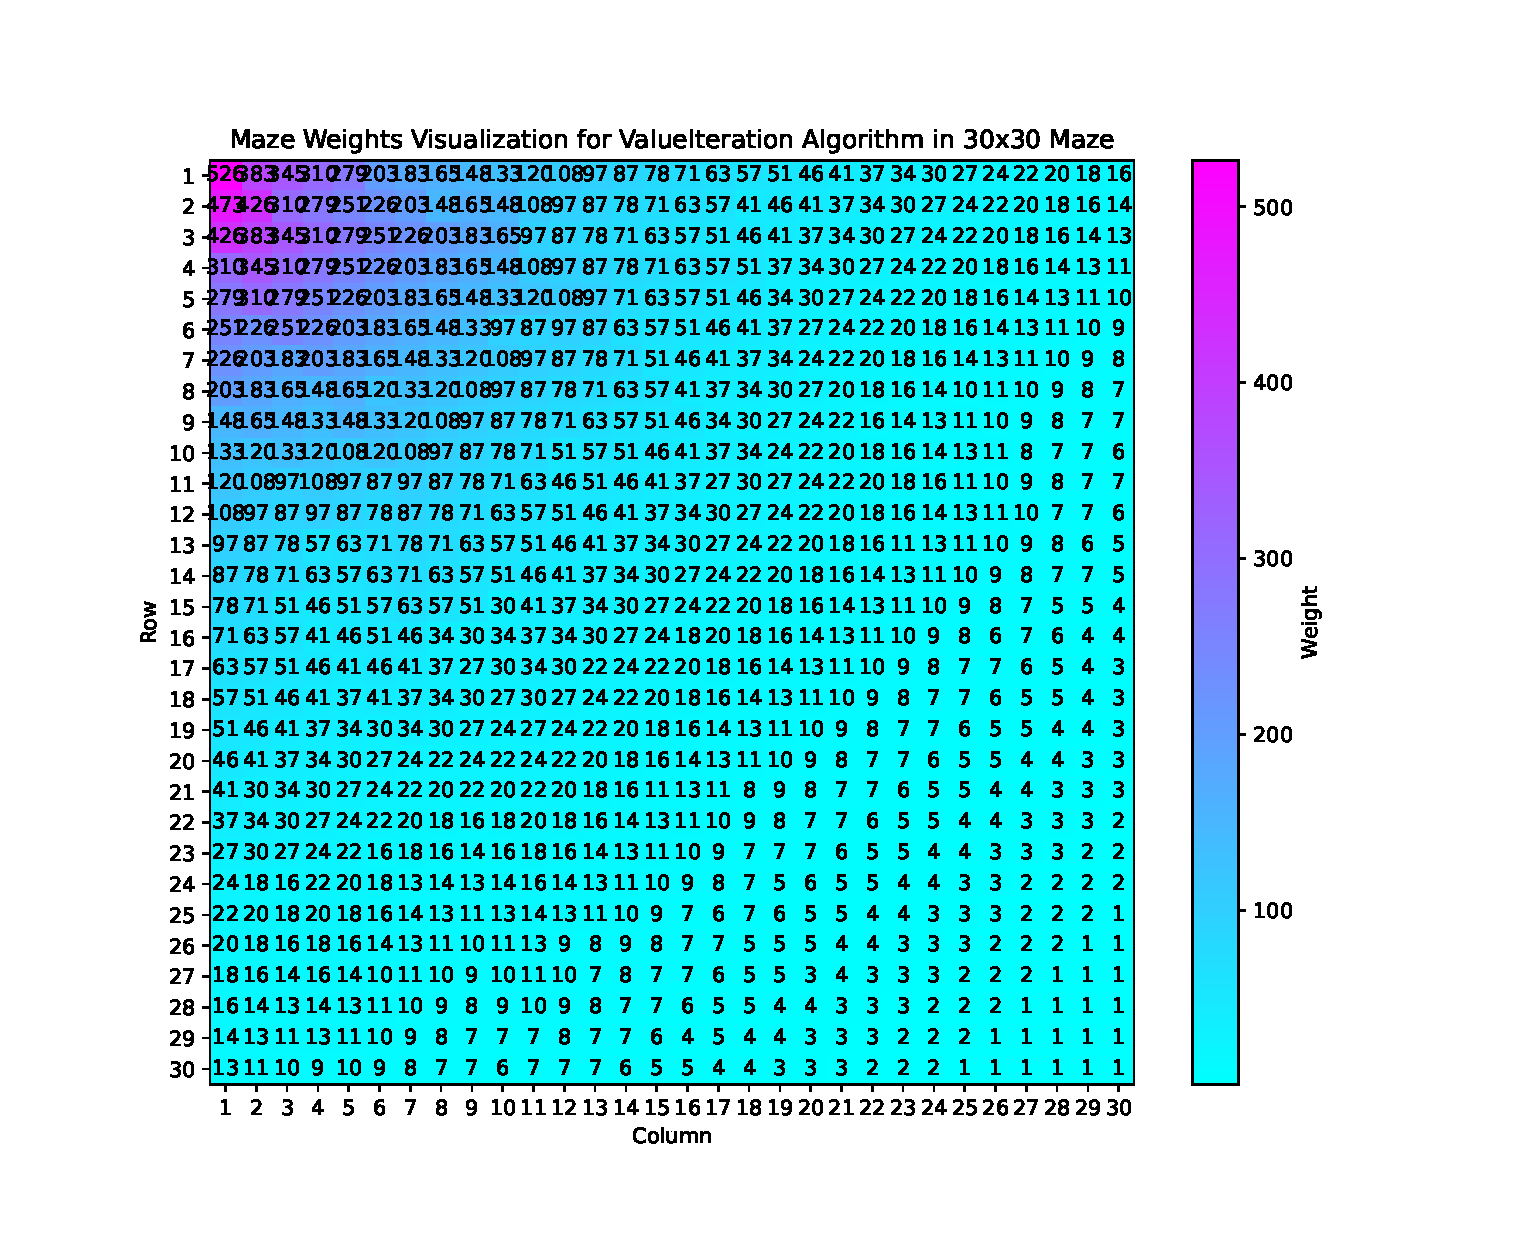
\includegraphics[width=\textwidth]{imgs/ValueIteration-30-30.eps}
        \caption{30x30 Value Iteration}
    \end{subfigure}
    \begin{subfigure}[b]{0.48\textwidth}
        \centering
        \includegraphics[width=\textwidth]{imgs/PolicyIteration-30-30.eps}
        \caption{30x30 Policy Iteration}
    \end{subfigure}
    \newline
    \begin{subfigure}[b]{0.48\textwidth}
        \centering
        \includegraphics[width=\textwidth]{imgs/ValueIteration-50-50.eps}
        \caption{50x50 Value Iteration}
    \end{subfigure}
    \begin{subfigure}[b]{0.48\textwidth}
        \centering
        \includegraphics[width=\textwidth]{imgs/PolicyIteration-50-50.eps}
        \caption{50x50 Policy Iteration}
    \end{subfigure}
    \newline
    \caption{Heat Map of Markov Decision Process(1)}
\end{figure}

\begin{figure}[htp]
    \centering
    \begin{subfigure}[b]{1\textwidth}
        \centering
        \includegraphics[width=0.5\textwidth]{imgs/ValueIteration-50-100.eps}
        \caption{50x100 Value Iteration}
    \end{subfigure}
    \newline
    \begin{subfigure}[b]{1\textwidth}
        \centering
        \includegraphics[width=0.5\textwidth]{imgs/PolicyIteration-50-100.eps}
        \caption{50x100 Policy Iteration}
    \end{subfigure}
    \caption{Heat Map of Markov Decision Process(2)}
\end{figure}


\newpage
\section{Conclusion}
It can be concluded that it's important to consider which is the best algorithm in different situations.
For example, if the maze is small and the goal is to find the shortest path, A* and BFS is the best choice. 
In other words, before using an algorithm, it is necessary to analyze the requirements of the problem and determine the best solution.
Overall, Graph Search Algorithms are less time-consuming and Markov Decision Processes are more time-consuming.  
However, the Markov decision process consumes less memory when solving for the best goal.
DFS is the best choice if want to solve problems quickly and reduce memory and time overhead.

Overall, I got a lot from this assignment. Not only did I review the algorithms in detail, but I also reviewed OOP.

\section{Solution of the Maze by All the Algorithms}
This section is for showing the solutions of the selected maze by all the algorithms.

\begin{itemize}
    \item The path with arrow is the explored/searched path, and the path with line or dots is the final path.
    \item \texttt{Yellow} color represents the final path of the algorithm \texttt{BFS}.
    \item \texttt{Cyan} color (dark green) represents the final path of the algorithm \texttt{DFS}.
    \item \texttt{Green} color (light green) represents the final path of the algorithm \texttt{A*}.
    \item \texttt{Blue} color represents the final path of the algorithm \texttt{Value Iteration}.
    \item \texttt{Red} color represents the final path of the algorithm \texttt{Policy Iteration}.
\end{itemize}

\begin{figure}[htp]
    \centering
    \begin{subfigure}[b]{1\textwidth}
        \centering
        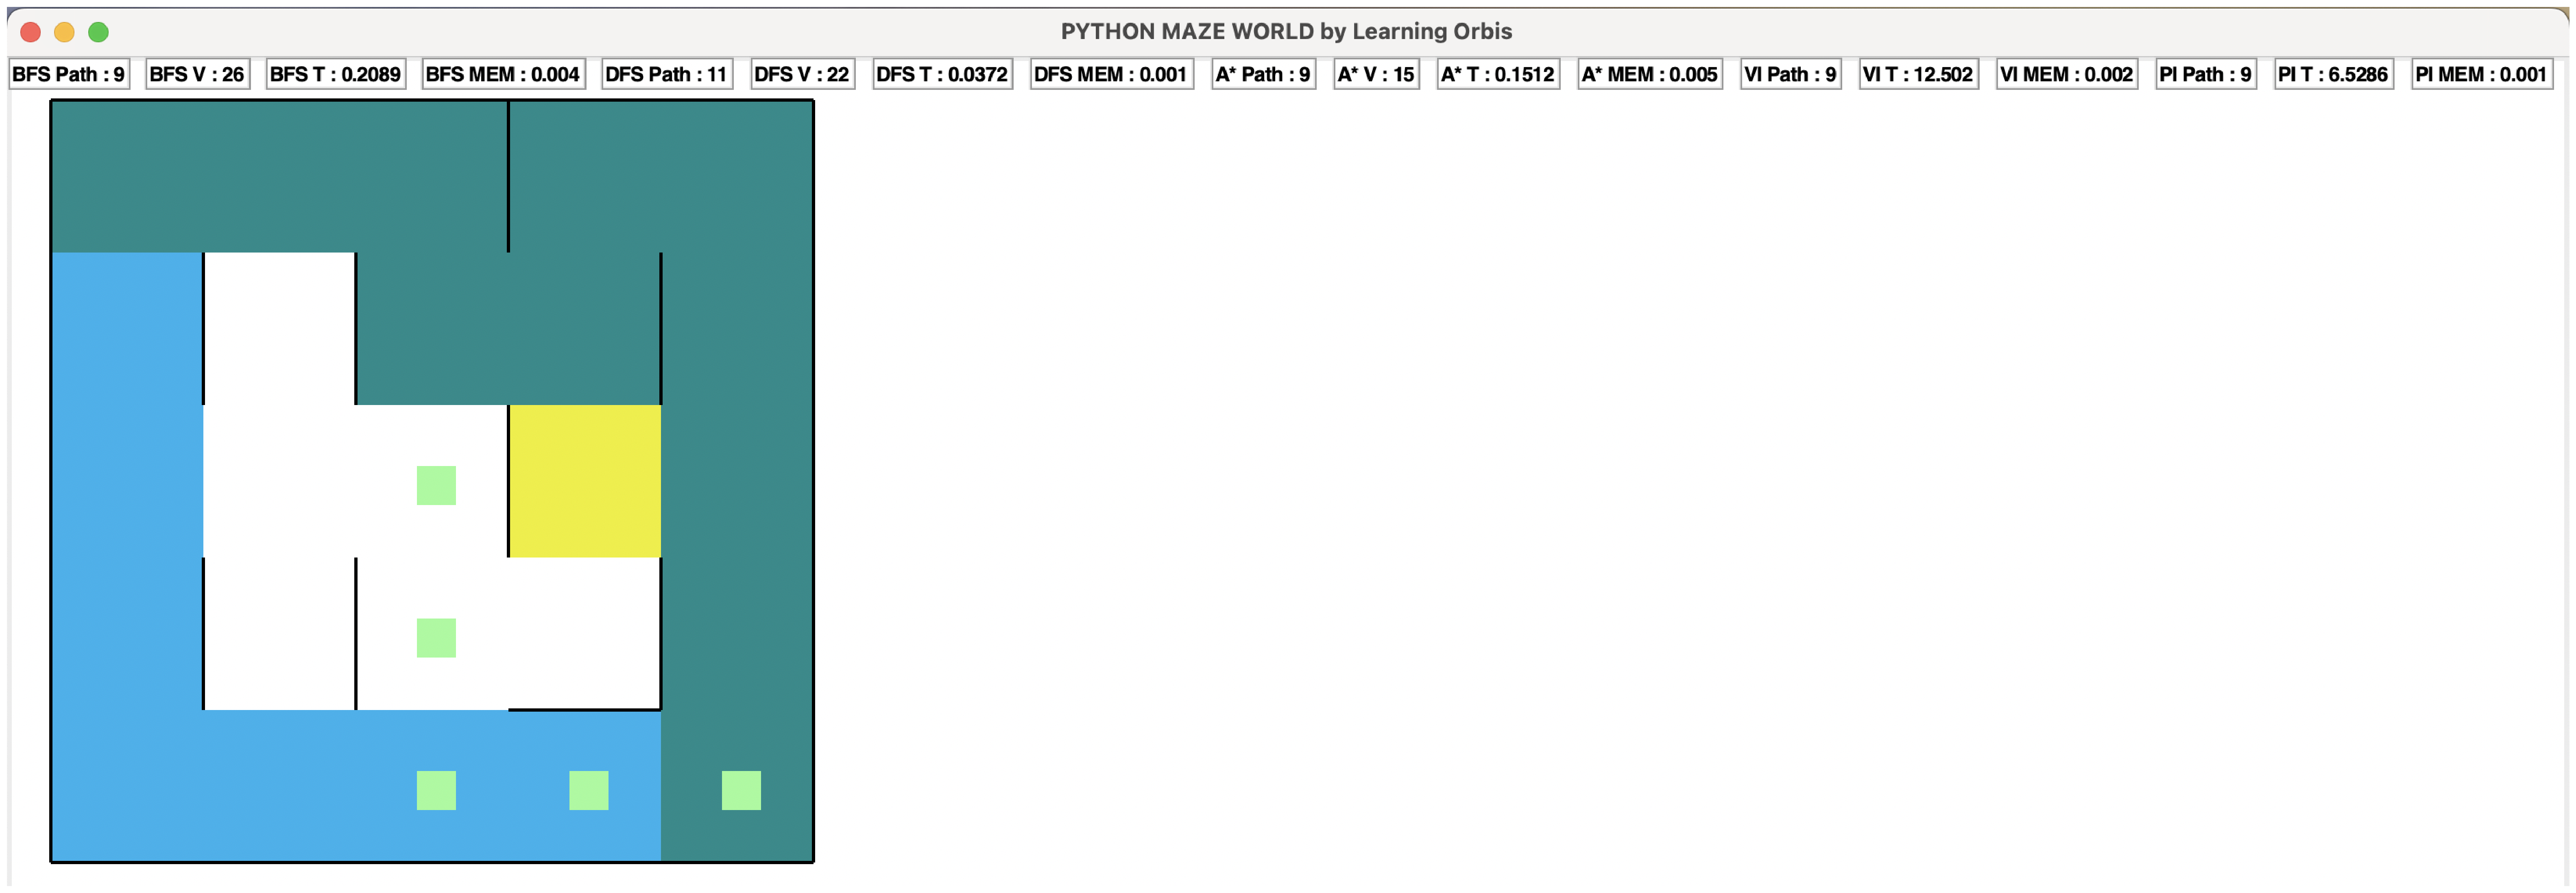
\includegraphics[width=\textwidth]{imgs/s_5.eps}
        \caption{5x5}
    \end{subfigure}
    \newline
    \begin{subfigure}[b]{1\textwidth}
        \centering
        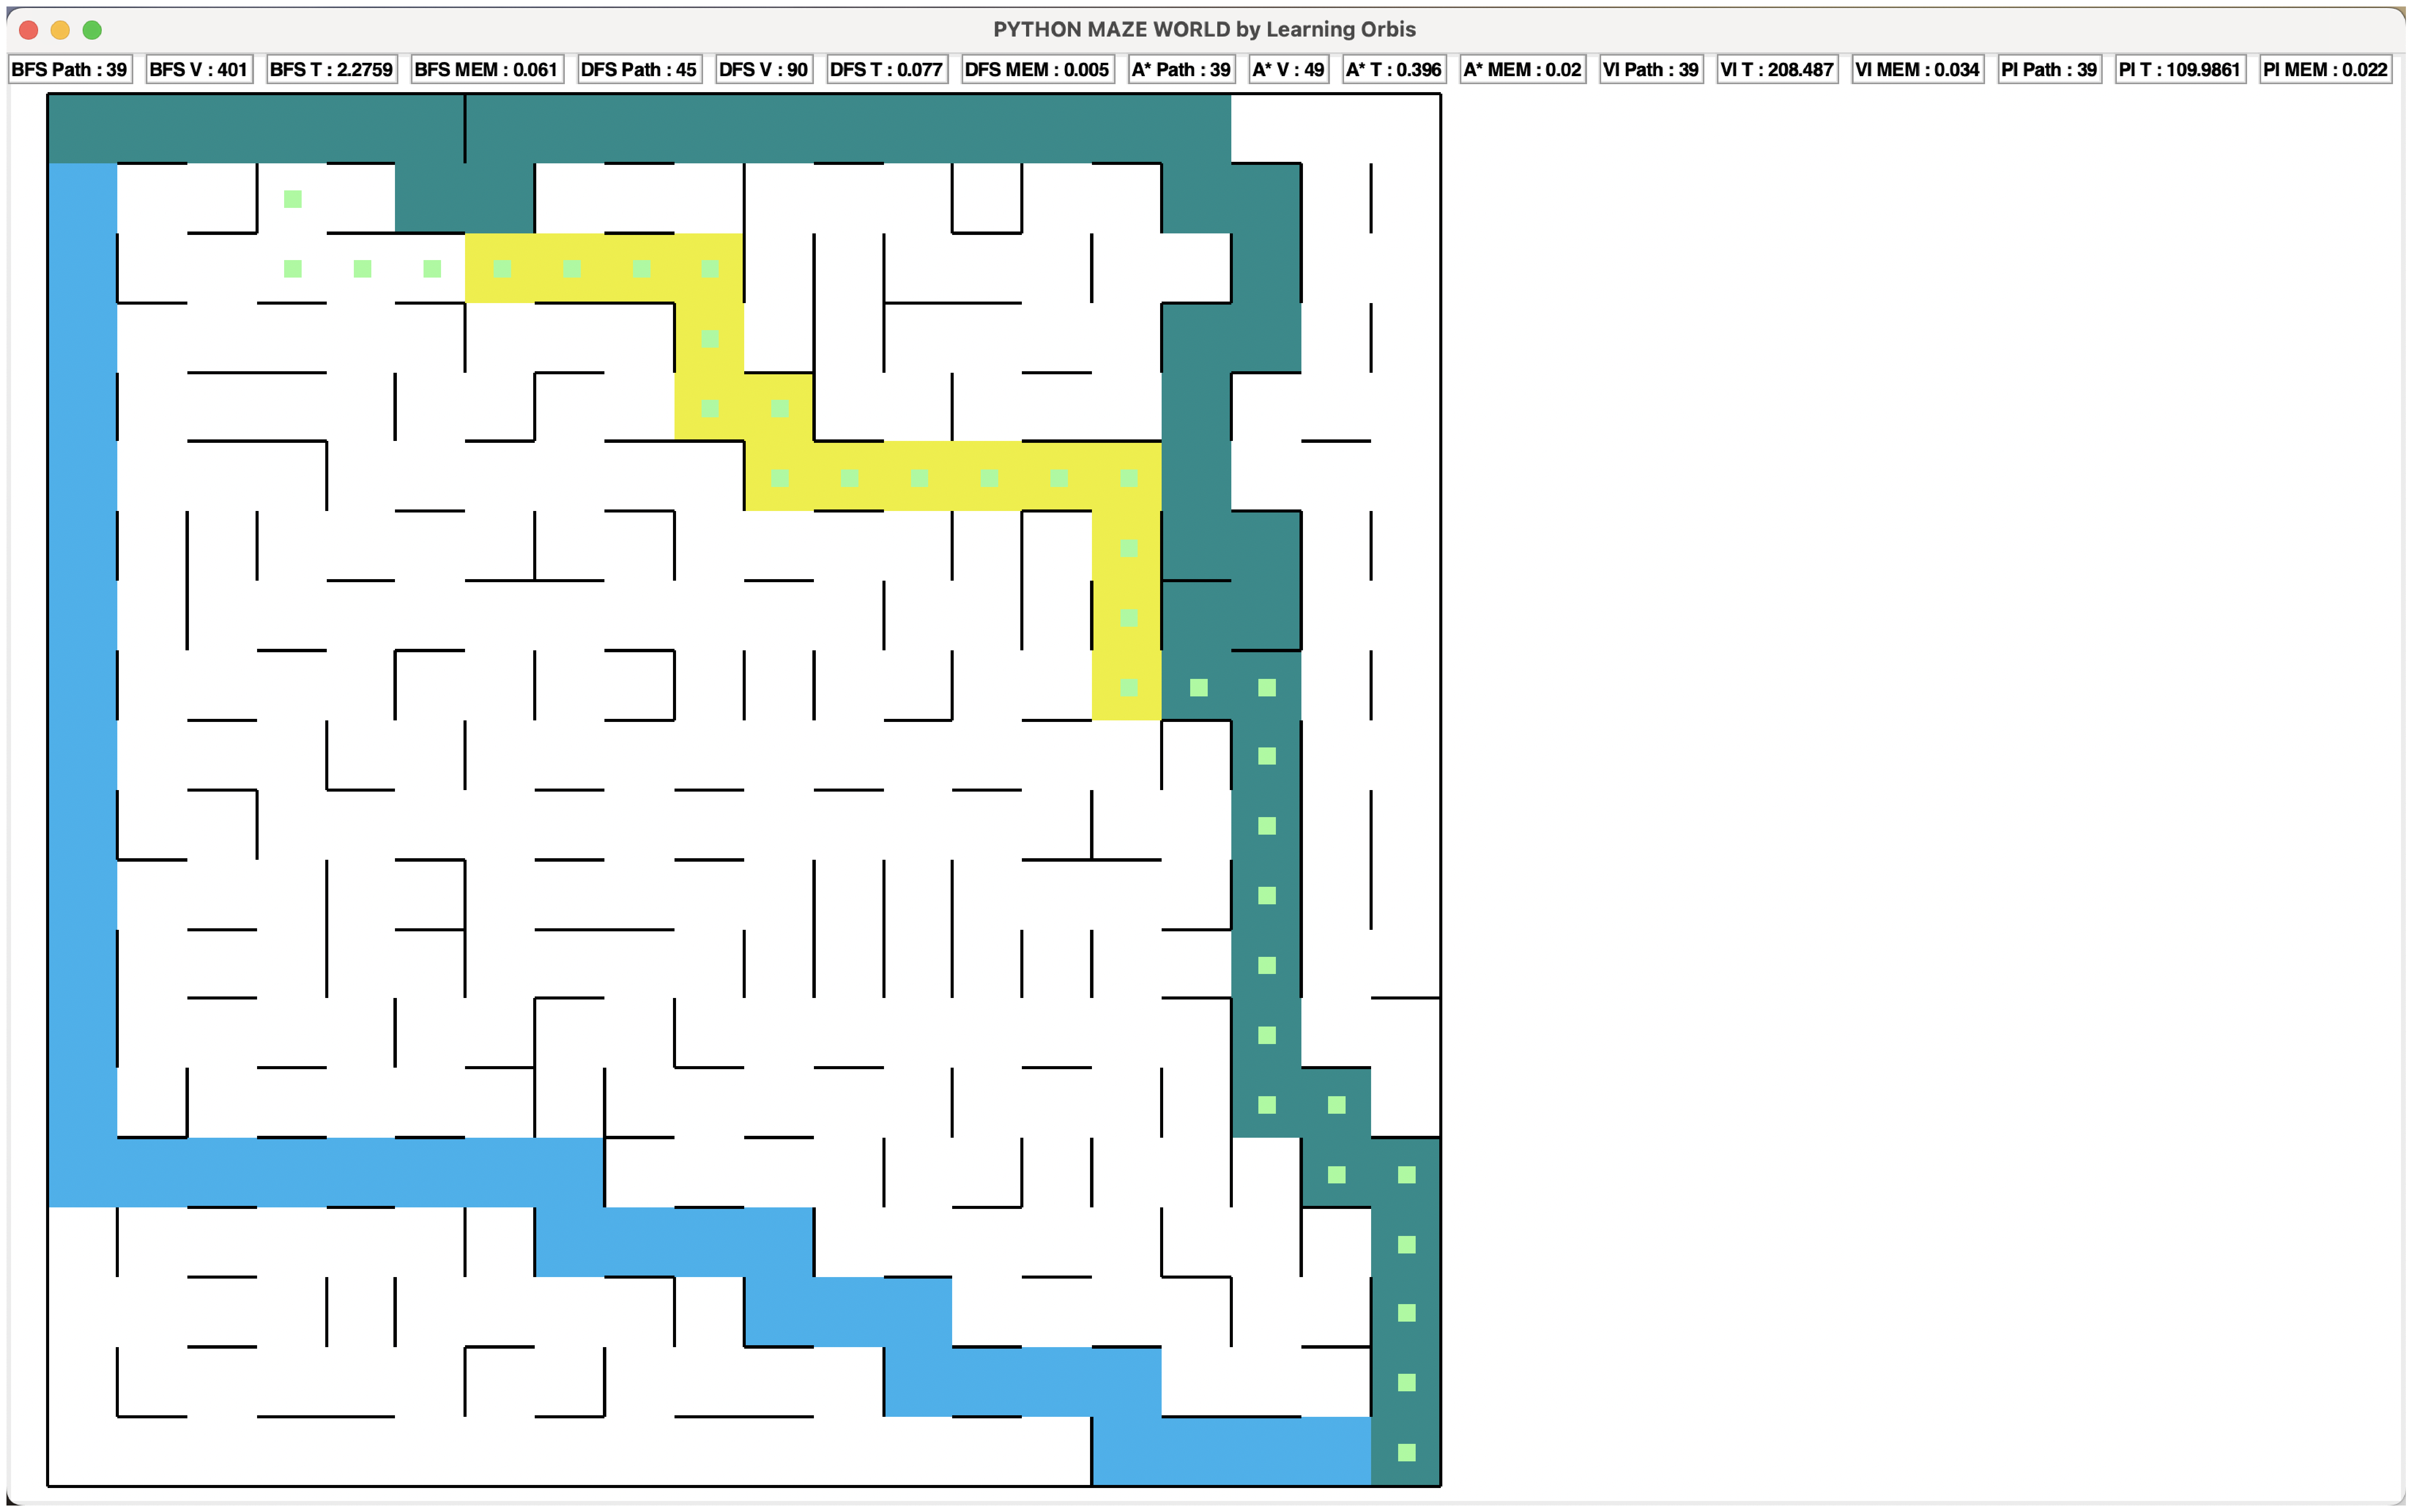
\includegraphics[width=\textwidth]{imgs/s_20.eps}
        \caption{20x20}
    \end{subfigure}
    \newline
    \begin{subfigure}[b]{1\textwidth}
        \centering
        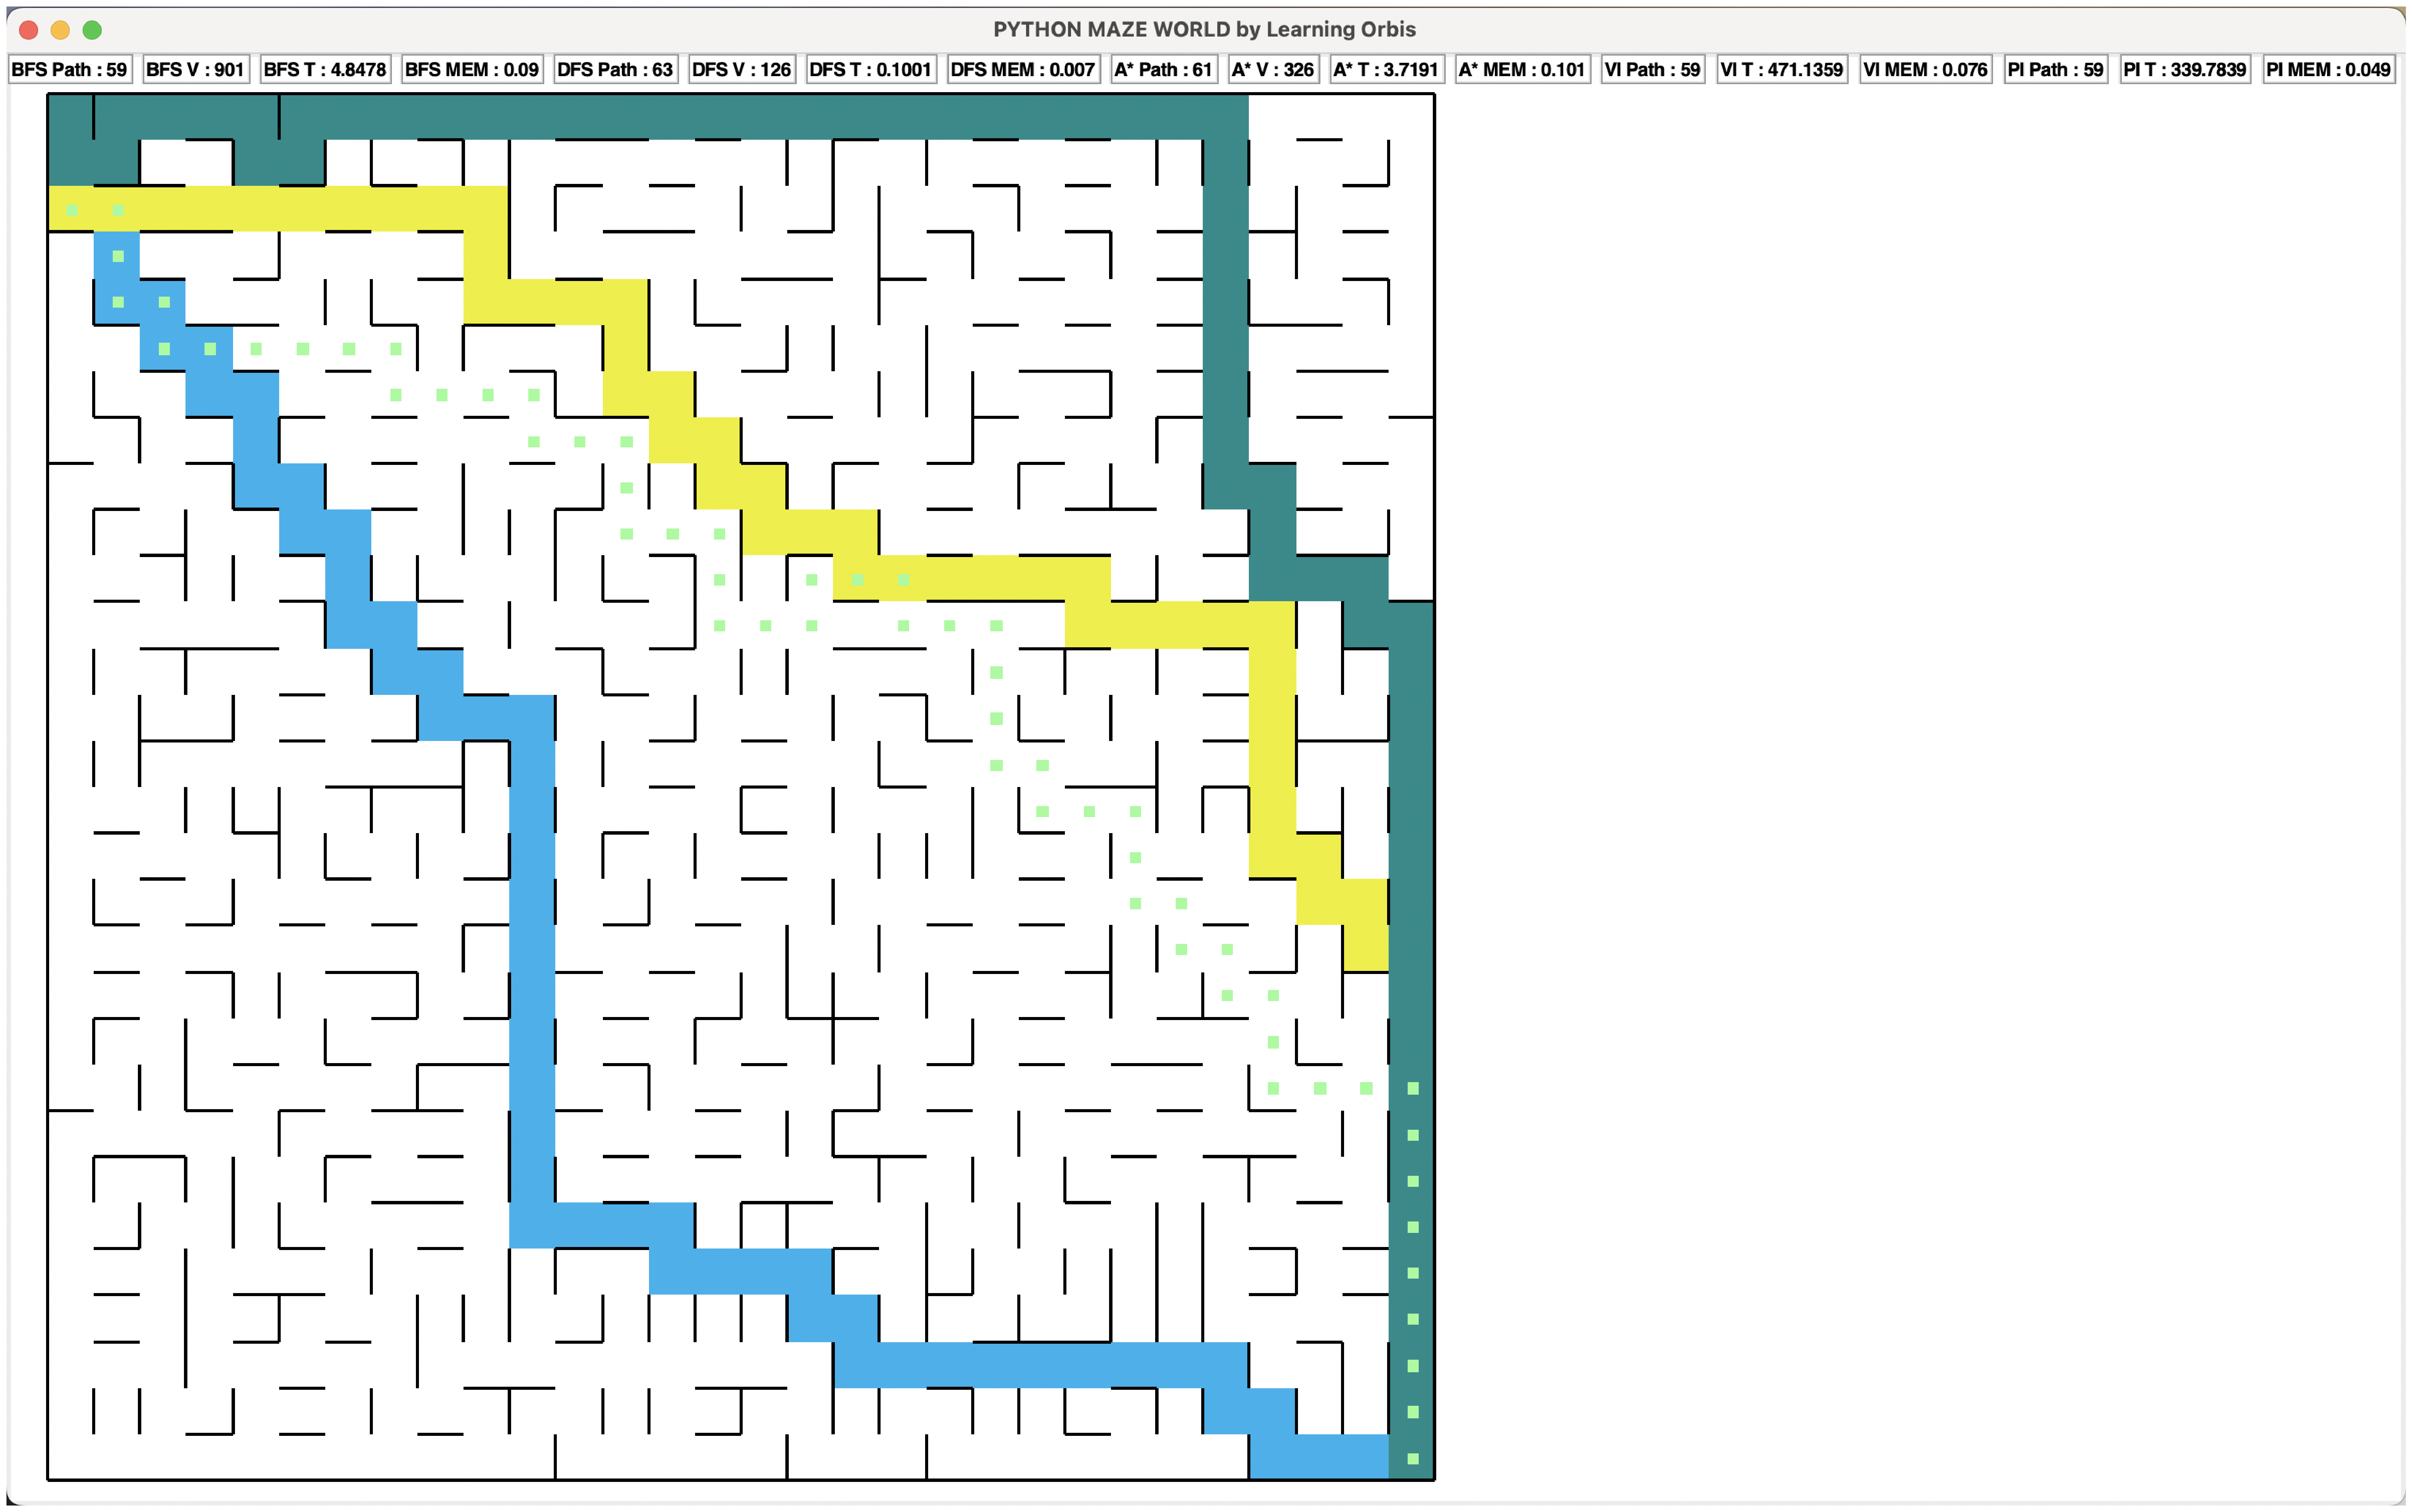
\includegraphics[width=\textwidth]{imgs/s_30.eps}
        \caption{30x30}
    \end{subfigure}
    \caption{Solutions of the Maze by All the Algorithms(1)}
\end{figure}

\begin{figure}[p]
    \centering
    \begin{subfigure}[b]{1\textwidth}
        \centering
        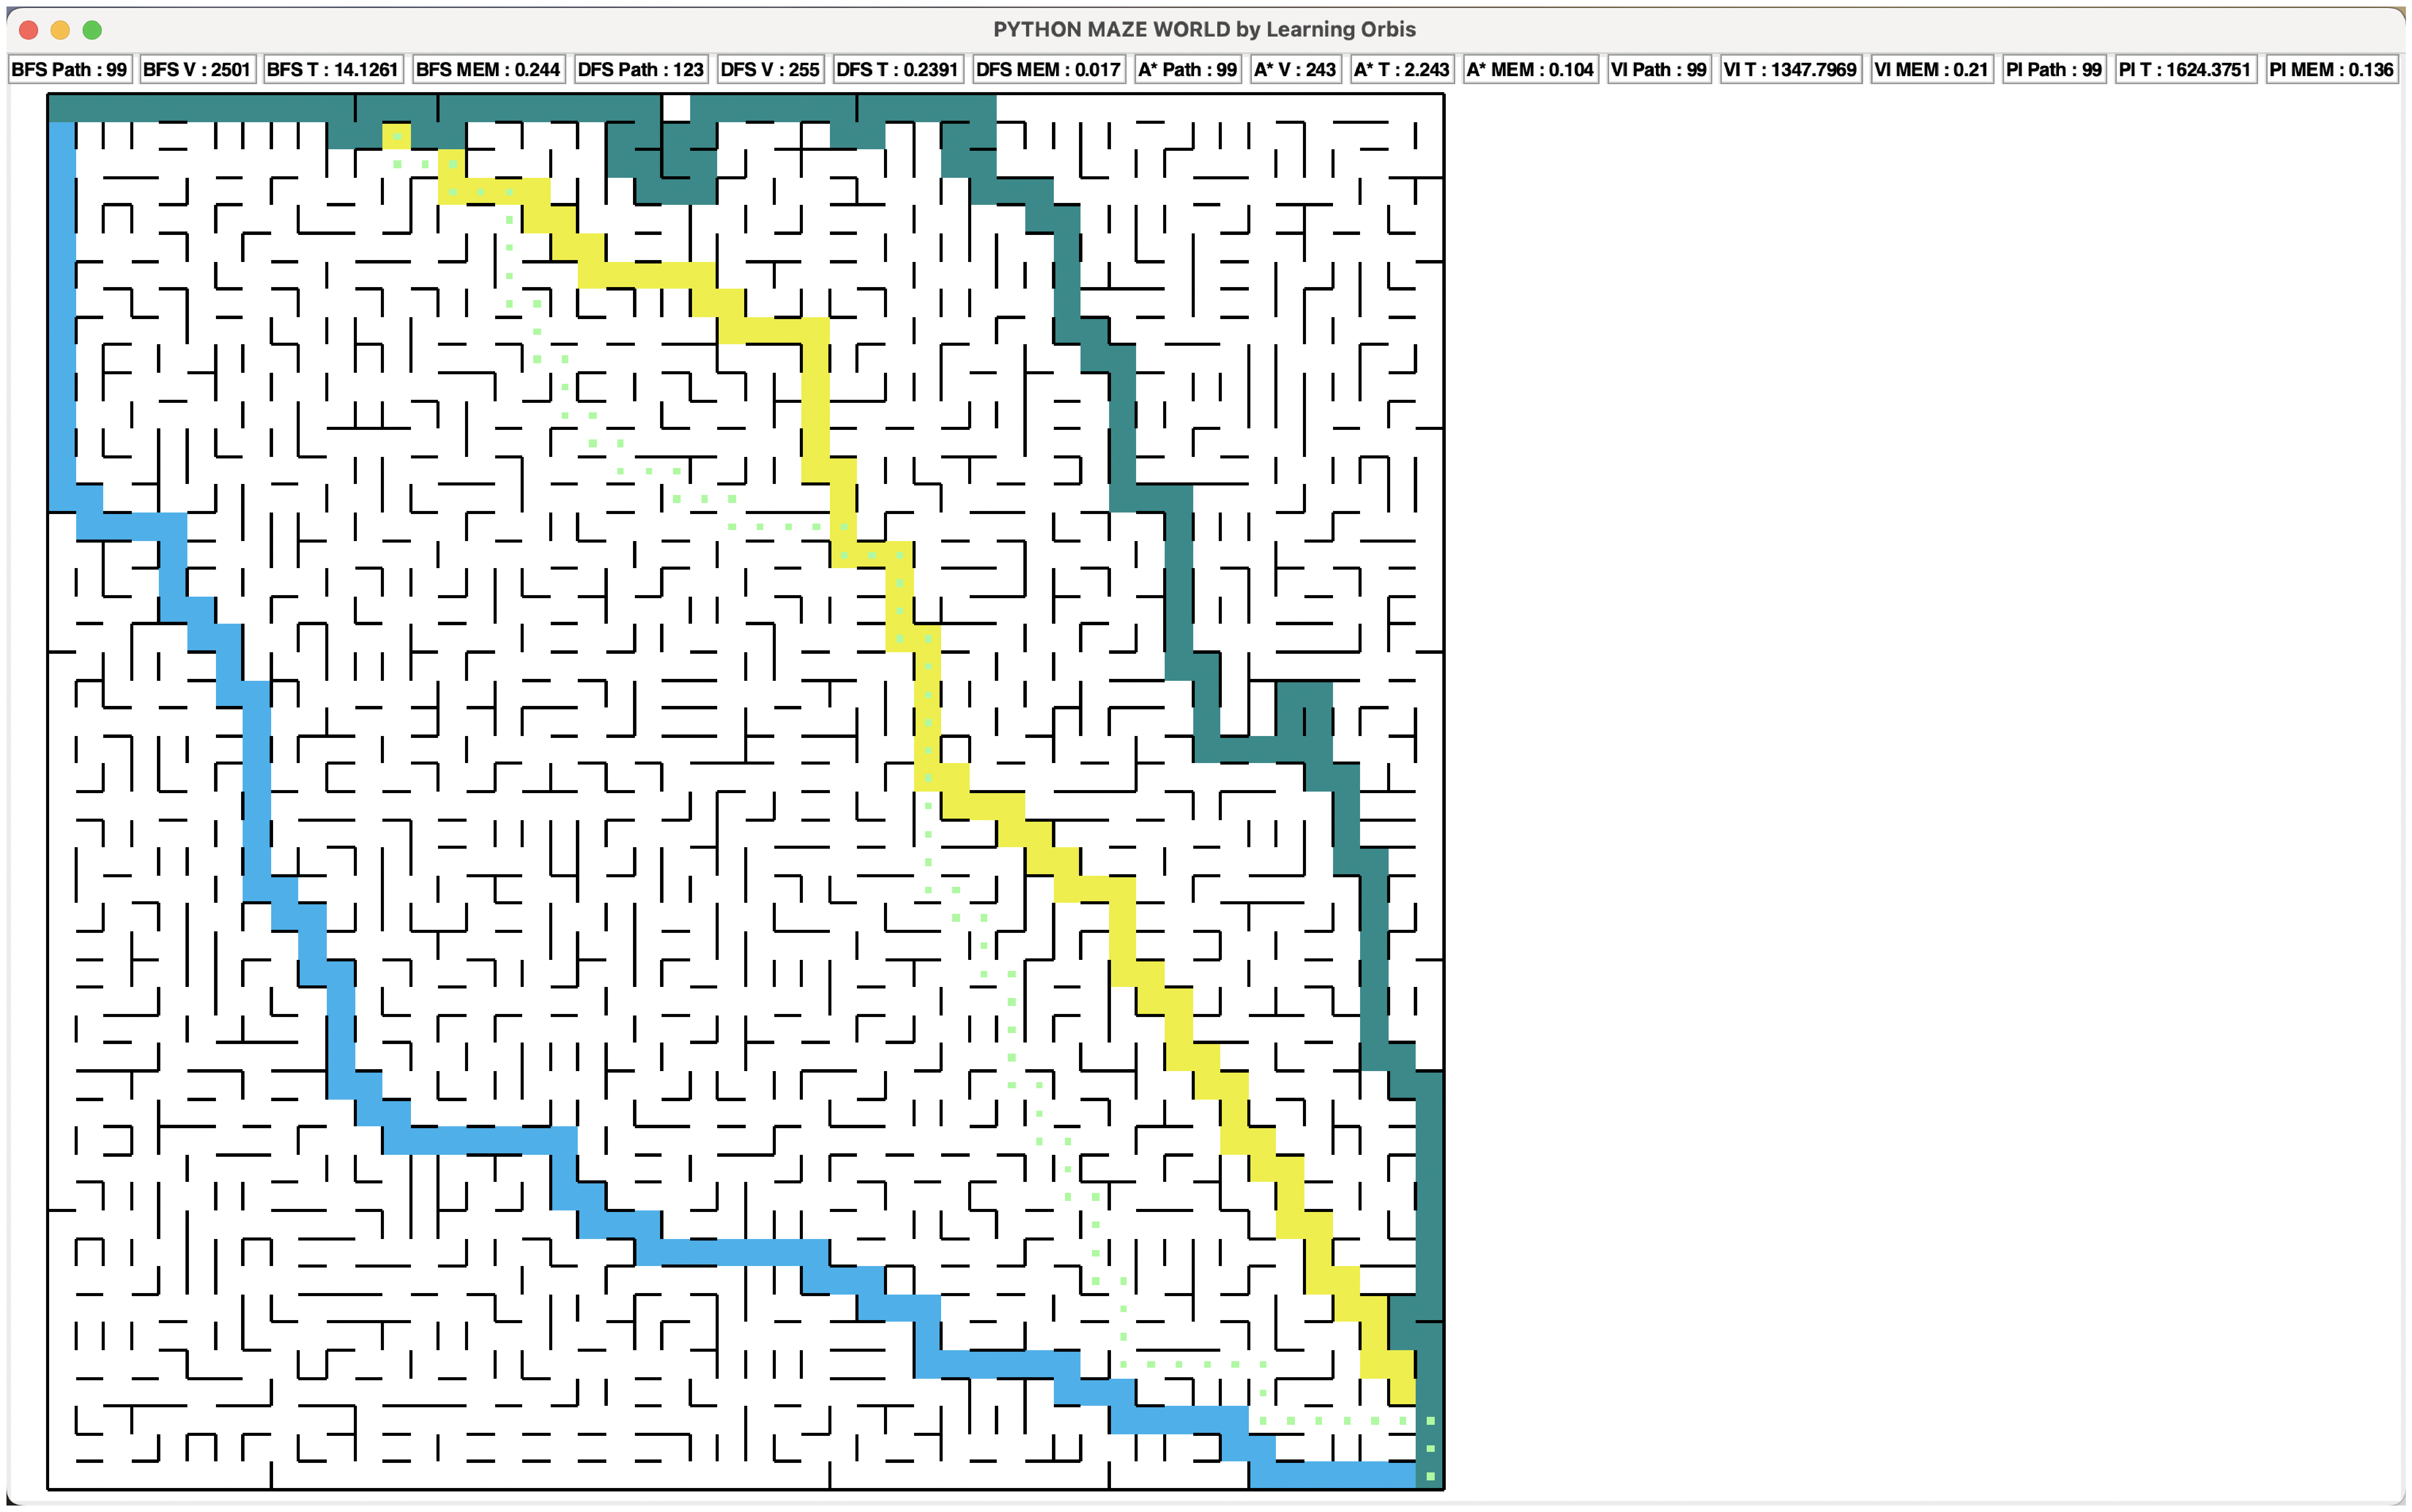
\includegraphics[width=1\textwidth]{imgs/s_50.eps}
        \caption{50x50}
    \end{subfigure}
    \newline
    \begin{subfigure}[b]{1\textwidth}
        \centering
        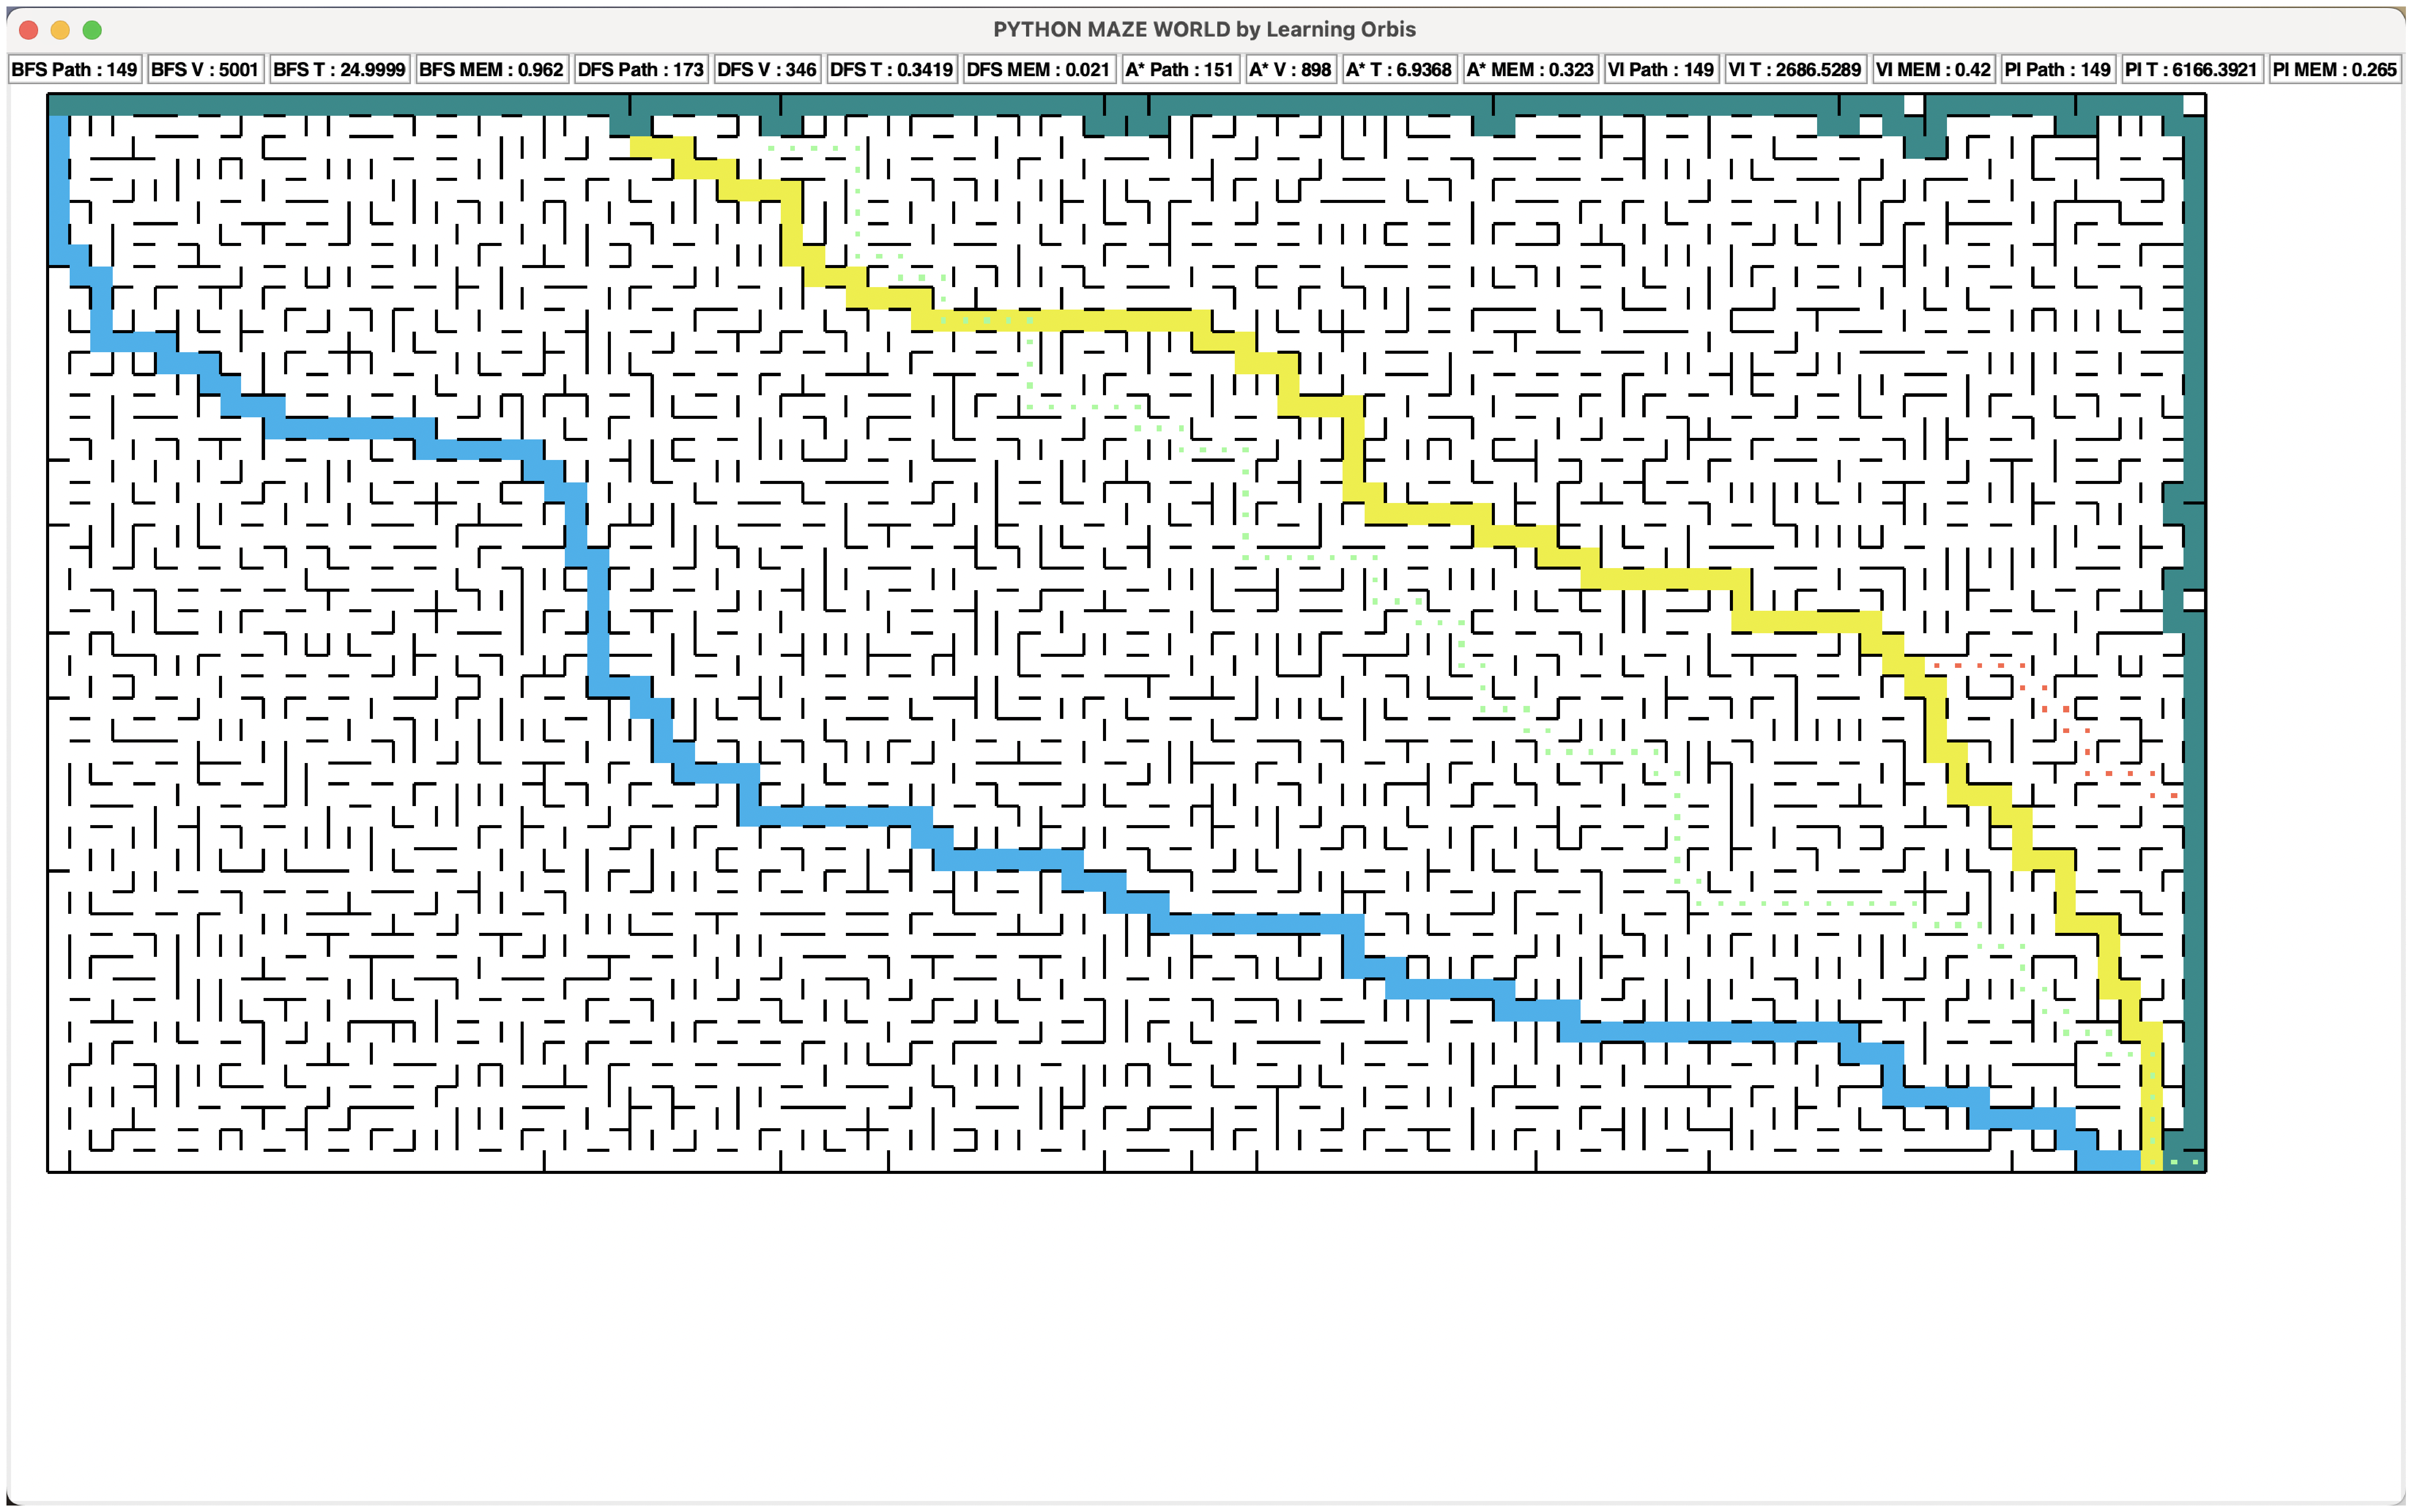
\includegraphics[width=1\textwidth]{imgs/s_50_100.eps}
        \caption{50x100}
    \end{subfigure}
    \caption{Solutions of the Maze by All the Algorithms(2)}
\end{figure}

\newpage
\bibliography{refs}
\bibliographystyle{ieeetr}
\newpage
\appendix
\section{Code of BFS}
\begin{lstlisting}
    from queue import Queue, PriorityQueue
    import time
    import tracemalloc as memory_trace
    from math import sqrt
    import numpy as np
    import matplotlib.pyplot as plt
    
    
    def start_memory_tracing():
        memory_trace.stop()
        memory_trace.start()
    
    
    class GraphSearchAlgorithms:
        def __init__(self, m, goal):
            self.m = m
            self.cost_time = 0
            self.memory_peak = 0
            self.goal = goal
            self.start_node = (self.m.rows, self.m.cols)
            self.visited = set()
            self.nodes = 'NWSE'
            self.final_path = []
            self.search_path = []
            self.origin_dict = {}
    
        def stop_memory_tracing(self):
            _, self.memory_peak = memory_trace.get_traced_memory()
            return self.memory_peak
    
        def validate_node(self, current_node):
            if current_node[0] < 1 or current_node[0] > self.m.rows or current_node[1] < 1 or current_node[1] > self.m.cols:
                return False
            if current_node in self.visited:
                return False
            return True
    
        def compute_next_node(self, current_node):
            for direction in self.nodes:
                if self.m.maze_map[current_node][direction]:
                    next_node = None
                    if direction == 'N':
                        next_node = (current_node[0] - 1, current_node[1])
                    elif direction == 'W':
                        next_node = (current_node[0], current_node[1] - 1)
                    elif direction == 'S':
                        next_node = (current_node[0] + 1, current_node[1])
                    elif direction == 'E':
                        next_node = (current_node[0], current_node[1] + 1)
                    if self.validate_node(next_node):
                        return next_node
    
        def traceback_final_path(self):
            final_path = []
            current_node = self.goal
            while current_node != self.start_node:
                final_path.append(current_node)
                current_node = self.origin_dict[current_node]
            final_path.append(self.start_node)
            return final_path[::-1]
    
        def execute_algorithm(self):
            pass
    
        def get_final_path(self):
            return self.final_path, len(self.search_path), self.cost_time, self.memory_peak
    
    
    class BFS(GraphSearchAlgorithms):
        def __init__(self, m, goal):
            super().__init__(m, goal)
            self.queue = Queue()
            self.queue.put(self.start_node)
    
        def execute_algorithm(self):
            start = time.time()
            start_memory_tracing()
            while self.queue:
                current_node = self.queue.get()
                self.search_path.append(current_node)
                if current_node == self.goal:
                    self.final_path = self.traceback_final_path()
                    end = time.time()
                    self.stop_memory_tracing()
                    self.cost_time = end - start
                    return self.search_path, self.final_path
                while True:
                    new_position = self.compute_next_node(current_node)
                    if new_position:
                        self.queue.put(new_position)
                        self.visited.add(new_position)
                        self.origin_dict[new_position] = current_node
                    else:
                        break
            return self.search_path, None
\end{lstlisting}
\section{Code of DFS}
\begin{lstlisting}
    from queue import Queue, PriorityQueue
    import time
    import tracemalloc as memory_trace
    from math import sqrt
    import numpy as np
    import matplotlib.pyplot as plt


    def start_memory_tracing():
        memory_trace.stop()
        memory_trace.start()


    class GraphSearchAlgorithms:
        def __init__(self, m, goal):
            self.m = m
            self.cost_time = 0
            self.memory_peak = 0
            self.goal = goal
            self.start_node = (self.m.rows, self.m.cols)
            self.visited = set()
            self.nodes = 'NWSE'
           self.final_path = []
           self.search_path = []
           self.origin_dict = {}

       def stop_memory_tracing(self):
           _, self.memory_peak = memory_trace.get_traced_memory()
           return self.memory_peak

       def validate_node(self, current_node):
          if current_node[0] < 1 or current_node[0] > self.m.rows or current_node[1] < 1 or current_node[1] > self.m.cols:
               return False
           if current_node in self.visited:
              return False
           return True

        def compute_next_node(self, current_node):
            for direction in self.nodes:
                if self.m.maze_map[current_node][direction]:
                    next_node = None
                    if direction == 'N':
                        next_node = (current_node[0] - 1, current_node[1])
                    elif direction == 'W':
                        next_node = (current_node[0], current_node[1] - 1)
                    elif direction == 'S':
                        next_node = (current_node[0] + 1, current_node[1])
                    elif direction == 'E':
                        next_node = (current_node[0], current_node[1] + 1)
                    if self.validate_node(next_node):
                        return next_node

        def traceback_final_path(self):
            final_path = []
            current_node = self.goal
            while current_node != self.start_node:
                final_path.append(current_node)
                current_node = self.origin_dict[current_node]
            final_path.append(self.start_node)
            return final_path[::-1]

        def execute_algorithm(self):
            pass

        def get_final_path(self):
            return self.final_path, len(self.search_path), self.cost_time, self.memory_peak

            class DFS(GraphSearchAlgorithms):
            def __init__(self, m, goal):
                super().__init__(m, goal)
                self.final_path = [self.start_node]
                self.search_path = [self.start_node]
        
            def execute_algorithm(self):
                start = time.time()
                start_memory_tracing()
                while self.final_path:
                    current_position = self.final_path.pop()
                    self.search_path.append(current_position)
                    if current_position == self.goal:
                        end = time.time()
                        self.stop_memory_tracing()
                        self.cost_time = end - start
                        self.final_path.append(current_position)
                        return self.search_path, self.final_path
                    self.visited.add(current_position)
                    new_position = self.compute_next_node(current_position)
                    if new_position:
                        self.final_path.append(current_position)
                        self.final_path.append(new_position)
                        self.search_path.append(new_position)
                return self.search_path, None
\end{lstlisting}
\section{Code of A*}
\begin{lstlisting}
    from queue import Queue, PriorityQueue
    import time
    import tracemalloc as memory_trace
    from math import sqrt
    import numpy as np
    import matplotlib.pyplot as plt
    
    
    def start_memory_tracing():
        memory_trace.stop()
        memory_trace.start()
    
    
    class GraphSearchAlgorithms:
        def __init__(self, m, goal):
            self.m = m
            self.cost_time = 0
            self.memory_peak = 0
            self.goal = goal
            self.start_node = (self.m.rows, self.m.cols)
            self.visited = set()
            self.nodes = 'NWSE'
            self.final_path = []
            self.search_path = []
            self.origin_dict = {}
    
        def stop_memory_tracing(self):
            _, self.memory_peak = memory_trace.get_traced_memory()
            return self.memory_peak
    
        def validate_node(self, current_node):
            if current_node[0] < 1 or current_node[0] > self.m.rows or current_node[1] < 1 or current_node[1] > self.m.cols:
                return False
            if current_node in self.visited:
                return False
            return True
    
        def compute_next_node(self, current_node):
            for direction in self.nodes:
                if self.m.maze_map[current_node][direction]:
                    next_node = None
                    if direction == 'N':
                        next_node = (current_node[0] - 1, current_node[1])
                    elif direction == 'W':
                        next_node = (current_node[0], current_node[1] - 1)
                    elif direction == 'S':
                        next_node = (current_node[0] + 1, current_node[1])
                    elif direction == 'E':
                        next_node = (current_node[0], current_node[1] + 1)
                    if self.validate_node(next_node):
                        return next_node
    
        def traceback_final_path(self):
            final_path = []
            current_node = self.goal
            while current_node != self.start_node:
                final_path.append(current_node)
                current_node = self.origin_dict[current_node]
            final_path.append(self.start_node)
            return final_path[::-1]
    
        def execute_algorithm(self):
            pass
    
        def get_final_path(self):
            return self.final_path, len(self.search_path), self.cost_time, self.memory_peak
    
    
            class AStar(GraphSearchAlgorithms):
            def __init__(self, m, goal):
                super().__init__(m, goal)
                self.g_score = {self.start_node: 0}
                self.priority_queue = PriorityQueue()
                self.manhattan_flag = True
        
            def h_score(self, node, manhattan=True):
                if manhattan:
                    return abs(node[0] - self.goal[0]) + abs(node[1] - self.goal[1])
                else:  # Euclidean
                    return sqrt(((node[0] - self.goal[0]) ** 2) + ((node[1] - self.goal[1]) ** 2))
        
            def execute_algorithm(self):
                start = time.time()
                start_memory_tracing()
                self.priority_queue.put((self.g_score[self.start_node] + self.h_score(self.start_node), self.start_node))
        
                while self.priority_queue:
                    _, current_position = self.priority_queue.get()
                    self.search_path.append(current_position)
                    if current_position == self.goal:
                        end = time.time()
                        self.stop_memory_tracing()
                        self.cost_time = end - start
                        self.final_path = self.traceback_final_path()
                        return self.search_path, self.final_path
                    self.visited.add(current_position)
                    while True:
                        new_position = self.compute_next_node(current_position)
                        if new_position:
                            self.g_score[new_position] = self.g_score[current_position] + 1
                            self.priority_queue.put((self.g_score[new_position] + self.h_score(new_position), new_position))
                            self.origin_dict[new_position] = current_position
                            self.visited.add(new_position)
                        else:
                            break
                return self.search_path, None
\end{lstlisting}
\section{Code of Value Iteration}
\begin{lstlisting}
    from queue import Queue, PriorityQueue
    import time
    import tracemalloc as memory_trace
    from math import sqrt
    import numpy as np
    import matplotlib.pyplot as plt
    def start_memory_tracing():
        memory_trace.stop()
        memory_trace.start()

    def get_direction(current_node):
        return max(current_node, key=current_node.get)

        class MarkovDecisionProcess:
        def __init__(self, m=None, goal=None):
            self.m = m
            self.cost_time = 0
            self.memory_peak = 0
            self.final_path = {}
            self.m = m
            if goal is None:
                raise AssertionError("Goal Cannot Be None")
            self.goal = goal
            self.start_node = (self.m.rows, self.m.cols)
    
            self.discount_factor = 0.9
            self.convergence_threshold = 0.000001
            self.transition_probability = {'N': 1, 'S': 1, 'W': 1, 'E': 1}
            self.transition_dictionary = {key: {subkey: 0 for subkey in self.m.maze_map[key]} for key in self.m.maze_map}
    
        def start_memory_tracing(self):
            memory_trace.stop()
            memory_trace.start()
    
        def stop_memory_tracing(self):
            _, self.memory_peak = memory_trace.get_traced_memory()
            return self.memory_peak
    
        def get_final_path(self):
            next_node = [self.start_node]
    
            while len(next_node) > 0:
                current_node = next_node.pop()
                if current_node == self.goal:
                    break
    
                direction = self.get_direction_for_current_node(current_node)
    
                if direction == 'N':
                    _temp_next_node_ = (current_node[0] - 1, current_node[1])
                elif direction == 'S':
                    _temp_next_node_ = (current_node[0] + 1, current_node[1])
                elif direction == 'W':
                    _temp_next_node_ = (current_node[0], current_node[1] - 1)
                elif direction == 'E':
                    _temp_next_node_ = (current_node[0], current_node[1] + 1)
                else:
                    raise AssertionError("Invalid Direction")
                self.final_path[current_node] = _temp_next_node_
                next_node.append(_temp_next_node_)
    
            return self.final_path, self.cost_time, self.memory_peak
    
        def get_direction_for_current_node(self, current_node):
            pass
    
        def execute_iteration(self):
            pass
    
        def plot_maze_weights(self):
            weights = np.zeros((self.m.rows, self.m.cols))
            data = self.transition_value
            for node, value in data.items():
                weights[node[0] - 1, node[1] - 1] = value
    
            plt.figure(figsize=(10, 8))
    
            if self.m.rows <= 30 and self.m.cols <= 30:
                for i in range(self.m.rows):
                    for j in range(self.m.cols):
                        if self.__class__.__name__ == 'ValueIteration':
                            if self.m.rows > 20 or self.m.cols > 20:
                                plt.text(j, i, str(int(weights[i, j])), ha='center', va='center', color='black')
                            else:
                                plt.text(j, i, format(weights[i, j], '.2f'), ha='center', va='center', color='black')
                        else:
                            if self.m.rows > 20 or self.m.cols > 20:
                                plt.text(j, i, format(weights[i, j], '.1f'), ha='center', va='center', color='black')
                            else:
                                plt.text(j, i, format(weights[i, j], '.4f'), ha='center', va='center', color='black')
    
            plt.imshow(weights, cmap='cool', interpolation='nearest', origin='upper')
            plt.colorbar(label='Weight')
            plt.xticks(np.arange(self.m.cols), np.arange(1, self.m.cols + 1))
            plt.yticks(np.arange(self.m.rows), np.arange(1, self.m.rows + 1))
            plt.title(f'Maze Weights Visualization for {self.__class__.__name__} Algorithm in {self.m.rows}x{self.m.cols} Maze')
            plt.xlabel('Column')
            plt.ylabel('Row')
            plt.show()
    
    
    class ValueIteration(MarkovDecisionProcess):
    
        def __init__(self, m=None, goal=None):
            super().__init__(m, goal)
            self.transition_value = {node: 10 if node == self.goal else 0 for node in self.m.grid}
            self.transition_reward = {node: 100 if node == self.goal else 0 for node in self.m.grid}
    
        def execute_iteration(self):
            start = time.time()
            self.start_memory_tracing()
            values_converged_flag = False
    
            while not values_converged_flag:
                values_converged_flag = True
    
                for current_node in self.m.grid:
                    temp_transition_value = []
    
                    for direction in ['N', 'S', 'W', 'E']:
                        if self.m.maze_map[current_node][direction] == 1:
                            try:
                                if direction == 'N':
                                    next_node = (current_node[0] - 1, current_node[1])
                                elif direction == 'S':
                                    next_node = (current_node[0] + 1, current_node[1])
                                elif direction == 'W':
                                    next_node = (current_node[0], current_node[1] - 1)
                                elif direction == 'E':
                                    next_node = (current_node[0], current_node[1] + 1)
                            except IndexError:
                                next_node = None
                            if next_node is not None:
                                next_transition_value = self.transition_probability[direction] * (
                                        self.transition_reward[current_node] +
                                        self.discount_factor * self.transition_value[next_node])
                                temp_transition_value.append(next_transition_value)
                                self.transition_dictionary[current_node][direction] = next_transition_value
                    best_transition_value = max(temp_transition_value)
    
                    if abs(best_transition_value - self.transition_value[current_node]) > self.convergence_threshold:
                        values_converged_flag = False
                        self.transition_value[current_node] = best_transition_value
    
            end = time.time()
            self.stop_memory_tracing()
            self.cost_time = end - start
    
        def get_direction_for_current_node(self, current_node):
            return get_direction(self.transition_dictionary[current_node])


\end{lstlisting}
\section{Code of Policy Iteration}
\begin{lstlisting}
    from queue import Queue, PriorityQueue
    import time
    import tracemalloc as memory_trace
    from math import sqrt
    import numpy as np
    import matplotlib.pyplot as plt
    def start_memory_tracing():
        memory_trace.stop()
        memory_trace.start()

    def get_direction(current_node):
        return max(current_node, key=current_node.get)

        class MarkovDecisionProcess:
        def __init__(self, m=None, goal=None):
            self.m = m
            self.cost_time = 0
            self.memory_peak = 0
            self.final_path = {}
            self.m = m
            if goal is None:
                raise AssertionError("Goal Cannot Be None")
            self.goal = goal
            self.start_node = (self.m.rows, self.m.cols)
    
            self.discount_factor = 0.9
            self.convergence_threshold = 0.000001
            self.transition_probability = {'N': 1, 'S': 1, 'W': 1, 'E': 1}
            self.transition_dictionary = {key: {subkey: 0 for subkey in self.m.maze_map[key]} for key in self.m.maze_map}
    
        def start_memory_tracing(self):
            memory_trace.stop()
            memory_trace.start()
    
        def stop_memory_tracing(self):
            _, self.memory_peak = memory_trace.get_traced_memory()
            return self.memory_peak
    
        def get_final_path(self):
            next_node = [self.start_node]
    
            while len(next_node) > 0:
                current_node = next_node.pop()
                if current_node == self.goal:
                    break
    
                direction = self.get_direction_for_current_node(current_node)
    
                if direction == 'N':
                    _temp_next_node_ = (current_node[0] - 1, current_node[1])
                elif direction == 'S':
                    _temp_next_node_ = (current_node[0] + 1, current_node[1])
                elif direction == 'W':
                    _temp_next_node_ = (current_node[0], current_node[1] - 1)
                elif direction == 'E':
                    _temp_next_node_ = (current_node[0], current_node[1] + 1)
                else:
                    raise AssertionError("Invalid Direction")
                self.final_path[current_node] = _temp_next_node_
                next_node.append(_temp_next_node_)
    
            return self.final_path, self.cost_time, self.memory_peak
    
        def get_direction_for_current_node(self, current_node):
            pass
    
        def execute_iteration(self):
            pass
    
        def plot_maze_weights(self):
            weights = np.zeros((self.m.rows, self.m.cols))
            data = self.transition_value
            for node, value in data.items():
                weights[node[0] - 1, node[1] - 1] = value
    
            plt.figure(figsize=(10, 8))
    
            if self.m.rows <= 30 and self.m.cols <= 30:
                for i in range(self.m.rows):
                    for j in range(self.m.cols):
                        if self.__class__.__name__ == 'ValueIteration':
                            if self.m.rows > 20 or self.m.cols > 20:
                                plt.text(j, i, str(int(weights[i, j])), ha='center', va='center', color='black')
                            else:
                                plt.text(j, i, format(weights[i, j], '.2f'), ha='center', va='center', color='black')
                        else:
                            if self.m.rows > 20 or self.m.cols > 20:
                                plt.text(j, i, format(weights[i, j], '.1f'), ha='center', va='center', color='black')
                            else:
                                plt.text(j, i, format(weights[i, j], '.4f'), ha='center', va='center', color='black')
    
            plt.imshow(weights, cmap='cool', interpolation='nearest', origin='upper')
            plt.colorbar(label='Weight')
            plt.xticks(np.arange(self.m.cols), np.arange(1, self.m.cols + 1))
            plt.yticks(np.arange(self.m.rows), np.arange(1, self.m.rows + 1))
            plt.title(f'Maze Weights Visualization for {self.__class__.__name__} Algorithm in {self.m.rows}x{self.m.cols} Maze')
            plt.xlabel('Column')
            plt.ylabel('Row')
            plt.show()
    
            class PolicyIteration(MarkovDecisionProcess):

            def __init__(self, m=None, goal=None):
                super().__init__(m, goal)
                self.transition_value = {node: 1 if node == self.goal else 0 for node in self.m.grid}
                self.transition_reward = {node: 1 if node == self.goal else 0 for node in self.m.grid}
                self.policy = {node: None if node == self.goal else 'N' for node in self.m.grid}
        
            def calculate_transition_value(self, current_node):
                _temp_transition_value_ = {'N': 0, 'S': 0, 'W': 0, 'E': 0}
                temp_node_transition_value = {current_node: _temp_transition_value_}
                for direction in ['N', 'S', 'W', 'E']:
                    if self.m.maze_map[current_node][direction] == 1:
                        next_node = None
                        try:
                            if direction == 'N':
                                next_node = (current_node[0] - 1, current_node[1])
                            elif direction == 'S':
                                next_node = (current_node[0] + 1, current_node[1])
                            elif direction == 'W':
                                next_node = (current_node[0], current_node[1] - 1)
                            elif direction == 'E':
                                next_node = (current_node[0], current_node[1] + 1)
                        except IndexError:
                            next_node = None
                        if next_node is not None:
                            next_transition_value = self.transition_value[next_node]
                        else:
                            next_transition_value = 0
        
                        temp_node_transition_value[current_node][direction] = self.transition_probability[direction] * (
                                self.transition_reward[current_node] +
                                self.discount_factor * next_transition_value)
                return temp_node_transition_value
        
            def execute_iteration(self):
                start = time.time()
                self.start_memory_tracing()
                value_converged_flag = False
                policy_converged_flag = False
        
                while not policy_converged_flag:
                    policy_converged_flag = True
                    value_converged_flag = False
                    while not value_converged_flag:
                        value_converged_flag = True
                        for current_node in self.m.grid:
                            if current_node == self.goal:
                                continue
                            current_policy = self.policy[current_node]
                            if self.m.maze_map[current_node][current_policy] == 1:
                                next_node = None
                                try:
                                    if current_policy == 'N':
                                        next_node = (current_node[0] - 1, current_node[1])
                                    elif current_policy == 'S':
                                        next_node = (current_node[0] + 1, current_node[1])
                                    elif current_policy == 'W':
                                        next_node = (current_node[0], current_node[1] - 1)
                                    elif current_policy == 'E':
                                        next_node = (current_node[0], current_node[1] + 1)
                                except IndexError:
                                    next_node = None
                                if next_node is not None:
                                    next_transition_value = self.transition_value[next_node]
                                else:
                                    next_transition_value = 0
        
                                self.transition_dictionary[current_node][current_policy] = (
                                        self.transition_probability[current_policy] * (
                                        self.transition_reward[current_node] +
                                        next_transition_value * self.discount_factor))
        
                                if abs(self.transition_value[current_node] - (self.transition_probability[current_policy] * (
                                        self.transition_reward[
                                            current_node] + next_transition_value * self.discount_factor))) > self.convergence_threshold:
                                    self.transition_value[current_node] = self.transition_probability[current_policy] * (
                                            self.transition_reward[
                                                current_node] + next_transition_value * self.discount_factor)
                                    value_converged_flag = False
                    for current_node in self.m.grid:
                        if current_node == self.goal:
                            continue
                        current_node_transition_value = self.calculate_transition_value(current_node)
                        current_node_transition_policy = get_direction(current_node_transition_value[current_node])
                        if current_node_transition_policy != self.policy[current_node]:
                            self.policy[current_node] = current_node_transition_policy
                            policy_converged_flag = False
        
                self.cost_time = time.time() - start
                self.stop_memory_tracing()
        
            def get_direction_for_current_node(self, current_node):
                return self.policy[current_node]
\end{lstlisting}
\section{Origin Data}
\begin{verbatim}
For 5x5 Maze:Path Lengths: {'BFS': 9, 'DFS': 11, 'A*': 9, 'VAL': 9, 'POL': 9}
Calculated Times: {'BFS': 0.2191, 'DFS': 0.0348, 'A*': 0.1507, 'VAL': 12.697, 'POL': 3.583}
Memory Consumptions: {'BFS': 0.004, 'DFS': 0.001, 'A*': 0.005, 'VAL': 0.002, 'POL': 0.002}
Visited Counts: {'BFS': 26, 'DFS': 22, 'A*': 15}

For 20x20 Maze:Path Lengths: {'BFS': 39, 'DFS': 45, 'A*': 39, 'VAL': 39, 'POL': 39}
Calculated Times: {'BFS': 2.3408, 'DFS': 0.1132, 'A*': 0.4311, 'VAL': 214.5798, 'POL': 102.3591}
Memory Consumptions: {'BFS': 0.061, 'DFS': 0.005, 'A*': 0.02, 'VAL': 0.034, 'POL': 0.022}
Visited Counts: {'BFS': 401, 'DFS': 90, 'A*': 49}

For 30x30 Maze:Path Lengths: {'BFS': 59, 'DFS': 63, 'A*': 61, 'VAL': 59, 'POL': 59}
Calculated Times: {'BFS': 5.2621, 'DFS': 0.1237, 'A*': 3.4239, 'VAL': 487.3381, 'POL': 334.6488}
Memory Consumptions: {'BFS': 0.09, 'DFS': 0.007, 'A*': 0.101, 'VAL': 0.076, 'POL': 0.049}
Visited Counts: {'BFS': 901, 'DFS': 126, 'A*': 326}

For 50x50 Maze:Path Lengths: {'BFS': 99, 'DFS': 123, 'A*': 99, 'VAL': 99, 'POL': 99}
Calculated Times: {'BFS': 13.545, 'DFS': 0.2058, 'A*': 2.1842, 'VAL': 1335.9559, 'POL': 1554.523}
Memory Consumptions: {'BFS': 0.244, 'DFS': 0.017, 'A*': 0.104, 'VAL': 0.21, 'POL': 0.136}
Visited Counts: {'BFS': 2501, 'DFS': 255, 'A*': 243}

For 50x100 Maze:Path Lengths: {'BFS': 149, 'DFS': 173, 'A*': 151, 'VAL': 149, 'POL': 149}
Calculated Times: {'BFS': 24.23, 'DFS': 0.3977, 'A*': 7.443, 'VAL': 2660.815, 'POL': 6087.6012}
Memory Consumptions: {'BFS': 0.962, 'DFS': 0.021, 'A*': 0.323, 'VAL': 0.42, 'POL': 0.265}
Visited Counts: {'BFS': 5001, 'DFS': 346, 'A*': 898}
\end{verbatim}
\section{License of pyamaze}
Link to pyamaze: \href{https://github.com/MAN1986/pyamaze}{pyamaze}
\begin{verbatim}
MIT License

Copyright (c) 2021 Muhammad Ahsan Naeem

Permission is hereby granted, free of charge, to any person obtaining a copy
of this software and associated documentation files (the "Software"), to deal
in the Software without restriction, including without limitation the rights
to use, copy, modify, merge, publish, distribute, sublicense, and/or sell
copies of the Software, and to permit persons to whom the Software is
furnished to do so, subject to the following conditions:

The above copyright notice and this permission notice shall be included in all
copies or substantial portions of the Software.

THE SOFTWARE IS PROVIDED "AS IS", WITHOUT WARRANTY OF ANY KIND, EXPRESS OR
IMPLIED, INCLUDING BUT NOT LIMITED TO THE WARRANTIES OF MERCHANTABILITY,
FITNESS FOR A PARTICULAR PURPOSE AND NONINFRINGEMENT. IN NO EVENT SHALL THE
AUTHORS OR COPYRIGHT HOLDERS BE LIABLE FOR ANY CLAIM, DAMAGES OR OTHER
LIABILITY, WHETHER IN AN ACTION OF CONTRACT, TORT OR OTHERWISE, ARISING FROM,
OUT OF OR IN CONNECTION WITH THE SOFTWARE OR THE USE OR OTHER DEALINGS IN THE
SOFTWARE.
\end{verbatim}
\section{License of matplotlib}
Link to matplotlib: \href{https://github.com/matplotlib/matplotlib}{Matplotlib}
\begin{verbatim}
    License agreement for matplotlib versions 1.3.0 and later
    =========================================================
    
    1. This LICENSE AGREEMENT is between the Matplotlib Development Team
    ("MDT"), and the Individual or Organization ("Licensee") accessing and
    otherwise using matplotlib software in source or binary form and its
    associated documentation.
    
    2. Subject to the terms and conditions of this License Agreement, MDT
    hereby grants Licensee a nonexclusive, royalty-free, world-wide license
    to reproduce, analyze, test, perform and/or display publicly, prepare
    derivative works, distribute, and otherwise use matplotlib
    alone or in any derivative version, provided, however, that MDT's
    License Agreement and MDT's notice of copyright, i.e., "Copyright (c)
    2012- Matplotlib Development Team; All Rights Reserved" are retained in
    matplotlib  alone or in any derivative version prepared by
    Licensee.
    
    3. In the event Licensee prepares a derivative work that is based on or
    incorporates matplotlib or any part thereof, and wants to
    make the derivative work available to others as provided herein, then
    Licensee hereby agrees to include in any such work a brief summary of
    the changes made to matplotlib .
    
    4. MDT is making matplotlib available to Licensee on an "AS
    IS" basis.  MDT MAKES NO REPRESENTATIONS OR WARRANTIES, EXPRESS OR
    IMPLIED.  BY WAY OF EXAMPLE, BUT NOT LIMITATION, MDT MAKES NO AND
    DISCLAIMS ANY REPRESENTATION OR WARRANTY OF MERCHANTABILITY OR FITNESS
    FOR ANY PARTICULAR PURPOSE OR THAT THE USE OF MATPLOTLIB
    WILL NOT INFRINGE ANY THIRD PARTY RIGHTS.
    
    5. MDT SHALL NOT BE LIABLE TO LICENSEE OR ANY OTHER USERS OF MATPLOTLIB
     FOR ANY INCIDENTAL, SPECIAL, OR CONSEQUENTIAL DAMAGES OR
    LOSS AS A RESULT OF MODIFYING, DISTRIBUTING, OR OTHERWISE USING
    MATPLOTLIB , OR ANY DERIVATIVE THEREOF, EVEN IF ADVISED OF
    THE POSSIBILITY THEREOF.
    
    6. This License Agreement will automatically terminate upon a material
    breach of its terms and conditions.
    
    7. Nothing in this License Agreement shall be deemed to create any
    relationship of agency, partnership, or joint venture between MDT and
    Licensee.  This License Agreement does not grant permission to use MDT
    trademarks or trade name in a trademark sense to endorse or promote
    products or services of Licensee, or any third party.
    
    8. By copying, installing or otherwise using matplotlib ,
    Licensee agrees to be bound by the terms and conditions of this License
    Agreement.
    
    License agreement for matplotlib versions prior to 1.3.0
    ========================================================
    
    1. This LICENSE AGREEMENT is between John D. Hunter ("JDH"), and the
    Individual or Organization ("Licensee") accessing and otherwise using
    matplotlib software in source or binary form and its associated
    documentation.
    
    2. Subject to the terms and conditions of this License Agreement, JDH
    hereby grants Licensee a nonexclusive, royalty-free, world-wide license
    to reproduce, analyze, test, perform and/or display publicly, prepare
    derivative works, distribute, and otherwise use matplotlib
    alone or in any derivative version, provided, however, that JDH's
    License Agreement and JDH's notice of copyright, i.e., "Copyright (c)
    2002-2011 John D. Hunter; All Rights Reserved" are retained in
    matplotlib  alone or in any derivative version prepared by
    Licensee.
    
    3. In the event Licensee prepares a derivative work that is based on or
    incorporates matplotlib  or any part thereof, and wants to
    make the derivative work available to others as provided herein, then
    Licensee hereby agrees to include in any such work a brief summary of
    the changes made to matplotlib.
    
    4. JDH is making matplotlib  available to Licensee on an "AS
    IS" basis.  JDH MAKES NO REPRESENTATIONS OR WARRANTIES, EXPRESS OR
    IMPLIED.  BY WAY OF EXAMPLE, BUT NOT LIMITATION, JDH MAKES NO AND
    DISCLAIMS ANY REPRESENTATION OR WARRANTY OF MERCHANTABILITY OR FITNESS
    FOR ANY PARTICULAR PURPOSE OR THAT THE USE OF MATPLOTLIB
    WILL NOT INFRINGE ANY THIRD PARTY RIGHTS.
    
    5. JDH SHALL NOT BE LIABLE TO LICENSEE OR ANY OTHER USERS OF MATPLOTLIB
     FOR ANY INCIDENTAL, SPECIAL, OR CONSEQUENTIAL DAMAGES OR
    LOSS AS A RESULT OF MODIFYING, DISTRIBUTING, OR OTHERWISE USING
    MATPLOTLIB , OR ANY DERIVATIVE THEREOF, EVEN IF ADVISED OF
    THE POSSIBILITY THEREOF.
    
    6. This License Agreement will automatically terminate upon a material
    breach of its terms and conditions.
    
    7. Nothing in this License Agreement shall be deemed to create any
    relationship of agency, partnership, or joint venture between JDH and
    Licensee.  This License Agreement does not grant permission to use JDH
    trademarks or trade name in a trademark sense to endorse or promote
    products or services of Licensee, or any third party.
    
    8. By copying, installing or otherwise using matplotlib,
    Licensee agrees to be bound by the terms and conditions of this License
    Agreement.
\end{verbatim}
\section{License of numpy}
Link to numpy: \href{https://github.com/MAN1986/pyamaze}{pyamaze}
\begin{verbatim}
    Copyright (c) 2005-2024, NumPy Developers.
All rights reserved.

Redistribution and use in source and binary forms, with or without
modification, are permitted provided that the following conditions are
met:

    * Redistributions of source code must retain the above copyright
       notice, this list of conditions and the following disclaimer.

    * Redistributions in binary form must reproduce the above
       copyright notice, this list of conditions and the following
       disclaimer in the documentation and/or other materials provided
       with the distribution.

    * Neither the name of the NumPy Developers nor the names of any
       contributors may be used to endorse or promote products derived
       from this software without specific prior written permission.

THIS SOFTWARE IS PROVIDED BY THE COPYRIGHT HOLDERS AND CONTRIBUTORS
"AS IS" AND ANY EXPRESS OR IMPLIED WARRANTIES, INCLUDING, BUT NOT
LIMITED TO, THE IMPLIED WARRANTIES OF MERCHANTABILITY AND FITNESS FOR
A PARTICULAR PURPOSE ARE DISCLAIMED. IN NO EVENT SHALL THE COPYRIGHT
OWNER OR CONTRIBUTORS BE LIABLE FOR ANY DIRECT, INDIRECT, INCIDENTAL,
SPECIAL, EXEMPLARY, OR CONSEQUENTIAL DAMAGES (INCLUDING, BUT NOT
LIMITED TO, PROCUREMENT OF SUBSTITUTE GOODS OR SERVICES; LOSS OF USE,
DATA, OR PROFITS; OR BUSINESS INTERRUPTION) HOWEVER CAUSED AND ON ANY
THEORY OF LIABILITY, WHETHER IN CONTRACT, STRICT LIABILITY, OR TORT
(INCLUDING NEGLIGENCE OR OTHERWISE) ARISING IN ANY WAY OUT OF THE USE
OF THIS SOFTWARE, EVEN IF ADVISED OF THE POSSIBILITY OF SUCH DAMAGE.
\end{verbatim}
\end{document}

\section{References}
The Impact of Anonymity in Online Communities
No Space for Reddit Spacing: Mapping the Reflexive Relationship Between Groups on 4chan and Reddit




